\documentclass{book}
\title{Definitions and Theorems in Computer Science}
\author{Willem Van Onsem\\\url{https://github.com/KommuSoft/publications}}
\date{Version 0.1.1}
\usepackage{amsthm,amsfonts,makeidx,draftwatermark,amssymb,MnSymbol,ifthen,tikz,subfigure}
\usepackage[nottoc,chapter,numbib,numindex]{tocbibind}
\usepackage[annataritalic]{tengwarscript}
\usepackage[hidelinks,pdfborder=0 0 0,pdfpagelabels,plainpages=false,linktocpage=false,pdfcreator={LaTeX}]{hyperref}
\SetWatermarkScale{7}
\usepackage[cm]{fullpage}
\makeindex

\newcommand{\negsim}{\mathop{\sim}} 
\DeclareRobustCommand\dashsim{\mathrel{|}\joinrel\mathrel{\smash{\sim}}}
\DeclareRobustCommand\negdashsim{\mathrel{|}\joinrel\mathrel{\smash{\negsim}}}

\newcommand{\cointerval}[2]{\ensuremath{\left[#1,#2\right[}}
\newcommand{\ocinterval}[2]{\ensuremath{\left]#1,#2\right]}}
\newcommand{\oointerval}[2]{\ensuremath{\left]#1,#2\right[}}
\newcommand{\ccinterval}[2]{\ensuremath{\left[#1,#2\right]}}
\newcommand{\dilemma}[1]{\brak{#1|\neg #1}}
\newcommand{\negdilemma}[1]{\brak{\neg #1|#1}}
\newcommand{\deflab}[1]{\label{def:#1}}
\newcommand{\defref}[1]{\textbf{ Definition \ref{def:#1}}}
\newcommand{\group}[1]{\ensuremath{\left\{\begin{array}{l}#1\end{array}\right.}}
\newcommand{\compclass}[1]{\textsc{\textbf{#1}}}
\newcommand{\bint}[4]{\ensuremath{\displaystyle\int_{#3}^{#4}{#1\ d#2}}}
\newcommand{\cd}{\ensuremath{\top\!\!\!\top}}
\newcommand{\ci}{\ensuremath{\bot\!\!\!\bot}}
\newcommand{\tuple}[1]{\ensuremath{\left\langle #1\right\rangle}}
\newcommand{\brak}[1]{\ensuremath{\left( #1\right)}}
\newcommand{\accol}[1]{\ensuremath{\left\{ #1\right\}}}
\newcommand{\flatbrak}[1]{\ensuremath{\left[ #1\right]}}

\newcommand{\fun}[2]{\ensuremath{#1\left(#2\right)}}
\newcommand{\funm}[2]{\fun{\mbox{#1}}{#2}}
\newcommand{\ffun}[1]{\fun{f}{#1}}
\newcommand{\gfun}[1]{\fun{g}{#1}}
\newcommand{\pfun}[1]{\fun{p}{#1}}
\newcommand{\Pfun}[1]{\fun{P}{#1}}
\newcommand{\pcond}[2]{\pfun{#1|#2}}
\newcommand{\funf}[2]{\ensuremath{#1\left[#2\right]}}

\newcommand{\sqnc}[3]{\ensuremath{#1,#2,\ldots,#3}}

\newcommand{\dom}[1]{\fun{\mbox{dom}}{#1}}

\newcommand{\iffTx}{if and only if}
\newcommand{\wrtTx}{with respect to}
\newcommand{\stTx}{such that}
\newcommand{\faTx}{for all}

\newcommand{\txIf}{\ensuremath{\mbox{If }}}
\newcommand{\txthen}{\ensuremath{\mbox{ then }}}
\newcommand{\txwhereas}{\ensuremath{\mbox{ whereas }}}
\newcommand{\funsig}[3]{\ensuremath{#1:#2 \rightarrow #3}}
\newcommand{\abs}[1]{\ensuremath{\left|#1\right|}}
\newcommand{\dtime}[1]{\fun{\compclass{DTIME}}{#1}}
\newcommand{\ntime}[1]{\fun{\compclass{NTIME}}{#1}}
\newcommand{\bigoh}[1]{\fun{O}{#1}}
\newcommand{\bigomega}[1]{\fun{\Omega}{#1}}
\newcommand{\smallomega}[1]{\fun{\omega}{#1}}
\newcommand{\bigtheta}[1]{\fun{\Theta}{#1}}
\newcommand{\binary}{\ensuremath{\left\{0,1\right\}}}
\newcommand{\binarystrings}{\ensuremath{\left\{0,1\right\}^*}}
\newcommand{\btobfun}[1]{\funsig{#1}{\binarystrings}{\binarystrings}}
\newcommand{\btoblfun}[1]{\funsig{#1}{\binarystrings}{\binary}}
\newcommand{\smalloh}[1]{\fun{o}{#1}}
\newcommand{\gcdf}[1]{\fun{\mbox{gcd}}{#1}}
\newcommand{\phif}[1]{\fun{\phi}{#1}}
\newcommand{\ordf}[1]{\fun{\mbox{ord}}{#1}}
\newcommand{\neigh}[1]{\fun{\calN}{#1}}
\newcommand{\perm}[1]{\ensuremath{\mbox{Perm}^{#1}}}
\newcommand{\argmax}[2][]{\ensuremath{\displaystyle\mbox{argmax}_{#1}\left(#2\right)}}

\newcommand{\calA}{\ensuremath{\mathcal{A}}}
\newcommand{\calB}{\ensuremath{\mathcal{B}}}
\newcommand{\calC}{\ensuremath{\mathcal{C}}}
\newcommand{\calD}{\ensuremath{\mathcal{D}}}
\newcommand{\calE}{\ensuremath{\mathcal{E}}}
\newcommand{\calF}{\ensuremath{\mathcal{F}}}
\newcommand{\calG}{\ensuremath{\mathcal{G}}}
\newcommand{\calH}{\ensuremath{\mathcal{H}}}
\newcommand{\calI}{\ensuremath{\mathcal{I}}}
\newcommand{\calJ}{\ensuremath{\mathcal{J}}}
\newcommand{\calK}{\ensuremath{\mathcal{K}}}
\newcommand{\calL}{\ensuremath{\mathcal{L}}}
\newcommand{\calLcalP}{\ensuremath{\mathcal{L}_{\mathcal{P}}}}
\newcommand{\calM}{\ensuremath{\mathcal{M}}}
\newcommand{\calN}{\ensuremath{\mathcal{N}}}
\newcommand{\calO}{\ensuremath{\mathcal{O}}}
\newcommand{\calP}{\ensuremath{\mathcal{P}}}
\newcommand{\calQ}{\ensuremath{\mathcal{Q}}}
\newcommand{\calR}{\ensuremath{\mathcal{R}}}
\newcommand{\calS}{\ensuremath{\mathcal{S}}}
\newcommand{\calT}{\ensuremath{\mathcal{T}}}
\newcommand{\calU}{\ensuremath{\mathcal{U}}}
\newcommand{\calV}{\ensuremath{\mathcal{V}}}
\newcommand{\calW}{\ensuremath{\mathcal{W}}}
\newcommand{\calX}{\ensuremath{\mathcal{X}}}
\newcommand{\calY}{\ensuremath{\mathcal{Y}}}
\newcommand{\calZ}{\ensuremath{\mathcal{Z}}}

\newcommand{\frakA}{\ensuremath{\mathfrak{A}}}
\newcommand{\frakB}{\ensuremath{\mathfrak{B}}}
\newcommand{\frakC}{\ensuremath{\mathfrak{C}}}
\newcommand{\frakD}{\ensuremath{\mathfrak{D}}}
\newcommand{\frakE}{\ensuremath{\mathfrak{E}}}
\newcommand{\frakF}{\ensuremath{\mathfrak{F}}}
\newcommand{\frakG}{\ensuremath{\mathfrak{G}}}
\newcommand{\frakH}{\ensuremath{\mathfrak{H}}}
\newcommand{\frakI}{\ensuremath{\mathfrak{I}}}
\newcommand{\frakJ}{\ensuremath{\mathfrak{J}}}
\newcommand{\frakK}{\ensuremath{\mathfrak{K}}}
\newcommand{\frakL}{\ensuremath{\mathfrak{L}}}
\newcommand{\frakM}{\ensuremath{\mathfrak{M}}}
\newcommand{\frakN}{\ensuremath{\mathfrak{N}}}
\newcommand{\frakO}{\ensuremath{\mathfrak{O}}}
\newcommand{\frakP}{\ensuremath{\mathfrak{P}}}
\newcommand{\frakQ}{\ensuremath{\mathfrak{Q}}}
\newcommand{\frakR}{\ensuremath{\mathfrak{R}}}
\newcommand{\frakS}{\ensuremath{\mathfrak{S}}}
\newcommand{\frakT}{\ensuremath{\mathfrak{T}}}
\newcommand{\frakU}{\ensuremath{\mathfrak{U}}}
\newcommand{\frakV}{\ensuremath{\mathfrak{V}}}
\newcommand{\frakW}{\ensuremath{\mathfrak{W}}}
\newcommand{\frakX}{\ensuremath{\mathfrak{X}}}
\newcommand{\frakY}{\ensuremath{\mathfrak{Y}}}
\newcommand{\frakZ}{\ensuremath{\mathfrak{Z}}}

\newcommand{\hats}{\ensuremath{\hat{s}}}
\newcommand{\soplus}{\ensuremath{\left\langle S,\oplus\right\rangle} }
\newcommand{\sotimes}{\ensuremath{\left\langle S,\otimes\right\rangle} }
\newcommand{\soplusotimes}{\ensuremath{\left\langle S,\oplus,\otimes\right\rangle} }
%\newcommand{\mod}{\ensuremath{\mbox{ mod }}}

\newcommand{\AAA}{\ensuremath{\mathbb{A}}}
\newcommand{\BBB}{\ensuremath{\mathbb{B}}}
\newcommand{\CCC}{\ensuremath{\mathbb{C}}}
\newcommand{\DDD}{\ensuremath{\mathbb{D}}}
\newcommand{\EEE}{\ensuremath{\mathbb{E}}}
\newcommand{\FFF}{\ensuremath{\mathbb{F}}}
\newcommand{\GGG}{\ensuremath{\mathbb{G}}}
\newcommand{\HHH}{\ensuremath{\mathbb{H}}}
\newcommand{\III}{\ensuremath{\mathbb{I}}}
\newcommand{\JJJ}{\ensuremath{\mathbb{J}}}
\newcommand{\KKK}{\ensuremath{\mathbb{K}}}
\newcommand{\LLL}{\ensuremath{\mathbb{L}}}
\newcommand{\MMM}{\ensuremath{\mathbb{M}}}
\newcommand{\NNN}{\ensuremath{\mathbb{N}}}
\newcommand{\OOO}{\ensuremath{\mathbb{O}}}
\newcommand{\PPP}{\ensuremath{\mathbb{P}}}
\newcommand{\QQQ}{\ensuremath{\mathbb{Q}}}
\newcommand{\RRR}{\ensuremath{\mathbb{R}}}
\newcommand{\SSS}{\ensuremath{\mathbb{S}}}
\newcommand{\TTT}{\ensuremath{\mathbb{T}}}
\newcommand{\UUU}{\ensuremath{\mathbb{U}}}
\newcommand{\VVV}{\ensuremath{\mathbb{V}}}
\newcommand{\WWW}{\ensuremath{\mathbb{W}}}
\newcommand{\XXX}{\ensuremath{\mathbb{X}}}
\newcommand{\YYY}{\ensuremath{\mathbb{Y}}}
\newcommand{\ZZZ}{\ensuremath{\mathbb{Z}}}

\newcommand{\nullmath}{\ensuremath{\mbox{\tt null}}}

\newcommand{\ZZZstarn}{\ensuremath{\ZZZ^*_n}}
\newcommand{\slHALT}{\mbox{\sl HALT}}
\newcommand{\slUC}{\mbox{\sl UC}}

\newcommand{\alg}[1]{\textsc{#1}}

\newtheorem{defi}{Definition}
\newtheorem{theo}{Theorem}

\newcommand{\term}[2][]{\ifthenelse{\equal{#1}{}}{{\bf #2}\index{#2}}{{\bf #2}\index{#1}}}
\newcommand{\termor}[2]{{\bf #1} (also called {\bf #2})\index{#1}\index{#2|see{#1}}}
\newcommand{\termabbrev}[2]{{\bf #1} (sometimes abbreviated as {\bf #2})\index{#1}\index{#2|see{#1}}}

\newcommand{\defiref}[1]{\textbf{\sc definition} \ref{def:#1}}

\begin{document}
\frontmatter
\begin{titlepage}
\maketitle
\end{titlepage}
\tableofcontents
\chapter*{Introduction}

\begin{defi}[Definition, Definiendum, Definiens]
A \term{definition} is a statement that explains the meaning of a term (a word, phrase, or other set of symbols). The term to be defined is the \term{definiendum}. The term may have many different senses and multiple meanings. For each meaning, a \term{definiens} is a cluster of words that defines that term (and clarifies the speaker's intention).
\cite{wiki:definition}
\end{defi}

This publication aims to compile a large number of common definitions and theorems in a single reference guide.

\section*{Advantage of a List of Definitions}

We expect the number of definitions in computer science to be around 100'000. The major problem with such definitions is that papers become quite inaccessible due to the fact that they use concepts who are defined elsewhere. This publication aims to tackle this problem by providing a collection of these definitions. Possible other advantages are a reduction of definition collisions: two meanings for the same term and preventing people from reinventing the wheel over and over again. A final advantage is that knowledge of a large amount of concepts enriches ones global understanding of computer science.

\section*{How is this Document Compiled?}

The definitions, theorems and lemma's are extracted from a massive amount of papers from conferences, proceedings, journals, etc. Since no individual can read this amount of papers in a lifetime, some intelligent scripts look for patterns who look interesting together with extracting the actual content. The extracted content is then reviewed by the author and after a minimal amount of modifications added to the right chapter.
\paragraph{}
The current processing rate is five definitions per day, but we hope by improving the data mining scripts, we will improve this number. At the moment our scripts already use optical character recognition together with error correction. We are currently working on technology that would be able to generate \LaTeX{} code for a specific formula.
\paragraph{}
People who want to help to improve the mining scripts, provide papers or do some post-processing can propose a pull-request on \url{http://goo.gl/jZeAG} or contact the author at \href{mailto:vanonsem.willem@gmail.com}{\nolinkurl{vanonsem.willem@gmail.com}}.

\mainmatter

\part{Mathematics, Theoretical Computer Science, Data Structures and Algorithms}
\chapter{Computation and Language}

\chapter{Computational Complexity}

\begin{defi}[Big-Oh notation]
If $f,g$ are two functions from $\NNN$ to $\NNN$, then we
\begin{enumerate}
 \item say that $f=\term{\bigoh{g}}$ if there exists a constant $c$ such that $\ffun{n}\leq c\gfun{n}$ for every sufficiently large $n$,
 \item say that $f=\term{\bigomega{g}}$ if $g = \bigoh{f}$,
 \item say that $f=\term{\bigtheta{g}}$ is $f = \bigoh{g}$ and $g = \bigoh{f}$,
 \item say that $f=\term{\smalloh{g}}$ if for every $\varepsilon>0$, $\ffun{n}\leq\varepsilon\gfun{n}$ for every sufficiently large $n$, and
 \item say that $f=\term{\smallomega{g}}$ if $g=\smalloh{f}$.
\end{enumerate}
\cite{arora2009computational}
\end{defi}

\begin{defi}[Computing a function and running time]
Let $\btobfun{f}$ and let $\funsig{T}{\NNN}{\NNN}$ be some functions, and let $M$ be a Turing machine. We say that $M$ \term{computes $f$} if for every $x\in\binarystrings$, whenever $M$ is initialized to the start configuration on input $x$, then it halts with $\ffun{x}$ written on its output tape. We say $M$ \term{computes $f$ in $\fun{T}{n}$-time} if its computation on every input $x$ requires at most $\fun{T}{\left|x\right|}$ steps.
\cite{arora2009computational}
\end{defi}

\begin{defi}[The class \compclass{DTIME}]
Let $\funsig{T}{\NNN}{\NNN}$ be some function. A language $L$ is in $\fun{\term{\compclass{DTIME}}}{\fun{T}{n}}$ if and only f there is a Turing machine that runs in time $c\fun{T}{n}$ for some constant $c>0$ and decides $L$.
\end{defi}

\begin{defi}[The class \compclass{P}]
\begin{equation}
\term{\compclass{P}}=\displaystyle\cup_{c\geq1}\fun{\compclass{DTIME}}{n^c}.
\end{equation}
\cite{arora2009computational}
\end{defi}

\begin{defi}[The class \compclass{NTIME}]
For every function $\funsig{T}{\NNN}{\NNN}$ and $L\subseteq\binarystrings$, we say that $L\in\fun{\term{\compclass{NTIME}}}{\fun{T}{n}}$ if there is a constant $c>0$ and a $c\fun{T}{n}$-time non deterministic Turing Machine $M$ such that for every $x\in\binarystrings$, $x\in L\leftrightarrow\fun{M}{x}=1$.
\cite{arora2009computational}
\end{defi}

\begin{defi}[The class \compclass{NP}]
\begin{equation}
\term{\compclass{NP}}=\displaystyle\cup_{c\geq1}\fun{\compclass{NTIME}}{n^c}.
\end{equation}
\cite{arora2009computational}
\end{defi}

\begin{defi}[Reduction, \compclass{NP-hard} and \compclass{NP-complete}]
A language $L\subseteq\binarystrings$ is \term{polynomial-time Karp reducible} to a language $L'\subseteq\binarystrings$ (sometimes shortened to just ``\term{polynomial-time reducible}''), denoted by $L\leq_p L'$, if there is a polynomial-time computable function $\btobfun{f}$ such that for every $x\in\binarystrings$, $x\in L$ if and only if $\ffun{x}\in L'$. We say that $L'$ is \term{\compclass{NP-hard}} if $L\leq_p L'$ for every $L\in\compclass{NP}$. We say that $L$ is \term{\compclass{NP-complete}} if $L'$ is \compclass{NP-hard} and $L'\in\compclass{NP}$.
\cite{arora2009computational}
\end{defi}

\begin{defi}[Complement language]
If $L\subseteq\binarystrings$ is a language, then we denote by $\overline{L}$ the \term{complement language} of $L$. That is, $\overline{L}=\binarystrings\setminus L$.
\cite{arora2009computational}
\end{defi}

\begin{defi}[The class \compclass{coNP}]
\begin{equation}
\term{\compclass{coNP}}=\left\{\overline{L}:L\in\compclass{NP}\right\}.
\end{equation}
\cite{arora2009computational}
\end{defi}

\begin{theo}[Efficient universal Turing machine]
\label{theo:eutm}
There exists a Turing Machine $\mathcal{U}$ such that for every $x,\alpha\in\binarystrings$, $\fun{\mathcal{U}}{x,\alpha} = \fun{M_{\alpha}}{x}$, where $M_{\alpha}$ denotes the Turing Machine represented by $\alpha$. Moreover, if $M_{\alpha}$ halts on input $x$ within $T$ steps then $\fun{\mathcal{U}}{x,\alpha}$ halts within $CT\log T$ steps, where $C$ is a number independent of $\left|x\right|$ and depending only on $M_{\alpha}$'s alphabet size, number of tapes, and number of states.
\cite{arora2009computational}
\end{theo}

\begin{theo}
\label{theo:uncomputable}There exists a function $\btoblfun{{\sf UC}}$ that is not computable by any Turing Machine.
\begin{proof}
The function $\sl UC$ is defined as follows: For every $\alpha\in\binarystrings$, if $\fun{M_{\alpha}}{\alpha}=1$, then $\fun{\sl UC}{\alpha}=0$; otherwise (if $\fun{M_{\alpha}}{\alpha}$ outputs a different value or enters an infinite loop), $\fun{\sl UC}{\alpha}=1$. Suppose for the sake of contradiction that ${\sl UC}$ is computable and hence there exists a Turing Machine $M$ such that $\fun{M}{\alpha}=\fun{{\sl UC}}{\alpha}$ for every $\alpha\in\binarystrings$. Then, in particular, $\fun{M}{\left\lfloor M\right\rfloor}=\fun{{\sl UC}}{\left\lfloor M\right\rfloor}$. But this is impossible: By the definition of ${\sl UC}$, $\fun{{\sl UC}}{\left\lfloor M\right\rfloor}=1\leftrightarrow\fun{M}{\left\lfloor M\right\rfloor}=1$.
\cite{arora2009computational}
\end{proof}
\end{theo}

\begin{theo}
{\slHALT} is not computable by any Turing Machine.
\begin{proof}
Suppose, for the sake of contradiction, that there was a Turing Machine $M_{\slHALT}$ computing $\slHALT$. We will use $M_{\slHALT}$ to show a Turing Machine $M_{\slUC}$ computing $\slUC$, contradicting Theorem \ref{theo:uncomputable}. The Turing Machine $M_{\slUC}$ is simple: On input $\alpha$, $M_{\slUC}$ runs $\fun{M_{\slHALT}}{\alpha,\alpha}$. If the result is 0 (meaning that $M_\alpha$ does not halt on $\alpha$), then $M_{\slUC}$ outputs $1$. Otherwise, $M_{\slUC}$ uses the universal Turing Machine $\mathcal{U}$ to compute $b=\fun{M_{\alpha}}{\alpha}$. If $b=1$, then $M_{\slUC}$ outputs $0$; otherwise, it outputs $1$. Under the assumption that $\fun{M_{\slHALT}}{\alpha,\alpha}$ outputs $\fun{\slHALT}{\alpha,\alpha}$ within a finite number of steps, the Turing Machine $\fun{M_{\slUC}}{\alpha}$ will output $\fun{\slUC}{\alpha}$.
\cite{arora2009computational}
\end{proof}
\end{theo}

\begin{theo}[\term{Time Hierarchy Theorem}]
\label{theo:tht}
If $f,g$ are time-constructible functions satisfying $\ffun{n}\log\ffun{n}=\smalloh{\gfun{n}}$, then
\begin{equation}
\dtime{\ffun{n}}\subsetneq\dtime{\gfun{n}}.
\end{equation}
\begin{proof}
To showcase the essential idea of the proof of Theorem \ref{theo:tht} with minimal notation, we prove the simpler statement $\dtime{n}\subsetneq\dtime{n^{1.5}}$. Consider the following Turing machine $D$: ``On input $x$, run for $\abs{x}^{1.4}$ steps the Universal Turing Machine $\mathcal{U}$ of Theorem \ref{theo:eutm} to simulate the execution of $M_x$ on $x$. If $\mathcal{U}$ outputs some bit $b\in\binary$ in this time, then output the opposite answer (i.e., output $1-b$). Else output 0.'' Here $M_x$ is the machine represented by the string $x$. By definition, $D$ halts within $n^{1.4}$ steps and hence the language $L$ decided by $D$ is in $\dtime{n^{1.5}}$. We claim that $L\notin\dtime{n}$. For contradiction's sake, assume that there is some Turing Machine $M$ and constant $c$ such that Turing Machine $M$, given any input $x\in\binarystrings$, halts within $c\abs{x}$ steps and outputs $\fun{D}{x}$. The time to simulate $M$ by the universal Turing machine $\mathcal{U}$ on every input x is at most $c'c\abs{
x}\log\abs{x}$ for some number $c'$ that depends on the alphabet size and number of tapes and states of $M$ but is independent of $\abs{x}$. There is some number $n_0$ such that $n^{1.4} > c'cn\log n$ for every $n\geq n_0$. Let $x$ be a string representing the machine $M$ whose length is at least $n_0$ (such a string exists since $M$ is represented by infinitely many strings). Then, $\fun{D}{x}$ will obtain the output $b=\fun{M}{x}$ within $\abs{x}^{1.4}$ steps, but by definition of $D$, we have $\fun{D}{x}=1-b=\fun{M}{x}$. Thus we have derived a contradiction. The proof Theorem \ref{theo:tht} for general $f,g$ is similar and uses the observation that the slowdown in simulating a machine using $\mathcal{U}$ is at most logarithmic.
\cite{arora2009computational}
\end{proof}
\end{theo}

\begin{theo}[\term{Nondeterministic Time Hierarchy Theorem}]
\label{theo:ndtht}
If $f,g$ are time constructible functions satisfying $\ffun{n+1}= \smalloh{\gfun{n}}$, then
\begin{equation}
\ntime{\ffun{n}}\subsetneq\ntime{\gfun{n}}.
\end{equation}
\begin{proof}
We just showcase the main idea by proving $\ntime{n}\subsetneq\ntime{n^{1.5}}$. The first instinct is to duplicate the proof of Theorem \ref{theo:tht}, since there is a universal Turing machine for nondeterministic computation as well. However, this alone does not suffice because the definition of the new machine $D$ requires the ability to ``flip the answer'', in other words, to efficiently compute, given the description of an nondeterminstic Turing machine $M$ and an input $x$, the value $1-\fun{M}{x}$. It is not obvious how to do this using the universal nondeterministic machine: it is unclear how a nondeterministic machine can just ``flip the answer''. Specifically, we do not expect that that the complement of an $\ntime{n}$ language will be in $\ntime{n^{1.5}}$. Now of course, the complement of every $\ntime{n}$ language is trivially decidable in exponential time (even deterministically) by examining all the
possibilities for the machine's nondeterministic choices, but on first sight this seems to be completely irrelevant to proving $\ntime{n}\subsetneq\ntime{n^{1.5}}$. Surprisingly, this trivial exponential simulation of a nondeterministic machine does suffice to establish a hierarchy theorem. The key idea will be lazy diagonalization, so named because the new machine $D$ is in no hurry to diagonalize and only ensures that it flips the answer of each linear time nondeterminstic Turing machine $M_i$ in only one string out of a sufficiently large (exponentially large) set of strings. Define the function $\funsig{f}{\NNN}{\NNN}$ as follows: $\ffun{1}=2$ and $\ffun{i+1}=2^{\ffun{i}^{1.2}}$. Given $n$, it's not hard to find in $\bigoh{n^1.5}$ time the number $i$ such that $n$ is sandwiched between $\ffun{i}$ and $\ffun{i+1}$. Our diagonalizing machine $D$ will try to flip the answer of $M_i$ on some input in the set $\left\{1^n:\ffun{i}<n\leq\ffun{i+1}\right\}$. $D$ is defined as follows:
\begin{quote}
``On input $x$, if $x\notin1^*$, reject. If $x=1^n$, then compute $i$ such that $\ffun{i}<n\leq\ffun{i+1}$ and
\begin{enumerate}
 \item If $\ffun{i}<n<\ffun{i+1}$ then simulate $M_i$ on input $1^{n+1}$ using nondeterminism in $n^{1.1}$ time and output its answer. (If $M_i$ has not halted in this time, then halt and accept.)
 \item If $n=\ffun{i+1}$, accept $1^n$ if and only if $M_i$ rejects $1^{\ffun{i}+1}$ in $(\ffun{i}+1)^{1.1}$ time.''
\end{enumerate}
\end{quote}
Part 2 requires going through all possible $2^(\ffun{i}+1)^{1.1}$ branches of $M_i$ on input $1^{\ffun{i}+1}$, but that is fine since the input size $\ffun{i+1}$ is $2^{\ffun{i}^{1.2}}$. Hence the nondeterminstic Turing machine $D$ runs in $\bigoh{n^{1.5}}$ time. Let $L$ be the language decided by $D$. We claim that $L\notin\ntime{n}$. Indeed, suppose for the sake of contradiction that $L$ is decided by an nondeterminstic Turing machine $M$ running in $cn$ steps (for some constant $c$). Since each nondeterminstic Turing machine is represented by infinitely many strings, we can find $i$ large enough such that $M=M_i$ and on inputs of length $n\geq\ffun{i}$, $M_i$ can be simulated in less than $n^{1.1}$ steps. This means that the two steps in the description of $D$ ensure, respectively, that

\begin{eqnarray}
\txIf\ffun{i}<n<\ffun{i+1},&\txthen\fun{D}{1^n}=\fun{M_i}{1^{n+1}}\label{eqn:ndtht33}\\
\txwhereas&\fun{D}{1^{\fun{f}{i+1}}}\neq\fun{M_i}{1^{\ffun{i}+1}}\label{eqn:ndtht34}
\end{eqnarray}

By our assumption $M_i$ and $D$ agree on all inputs $1^n$ for $n$ in the semi-open interval $\left(\ffun{i},\ffun{i+1}\right]$. Together with (\ref{eqn:ndtht33}), this implies that $\fun{D}{1^{\ffun{i+1}}}=\fun{M_i}{1^{\ffun{i}+1}}$, contradicting (\ref{eqn:ndtht34}).\cite{arora2009computational}
\end{proof}
\end{theo}
\chapter{Computational Geometry}

\chapter{Discrete Mathematics}

\section{Operator Properties}

\begin{defi}[Commutative operation]
A binary operation $\oplus$ is \term{commutative} if $a\oplus b = b\oplus a$ for all $a,b\in S$.\cite{Oppliger:2011:CC:2049860}
\end{defi}

\begin{defi}[Associative operation]
A binary operation $\oplus$ is \term{associative} if $a\oplus\left(b\oplus c\right) = \left(a\oplus b\right)\oplus c$ for all $a,b,c\in S$.\cite{Oppliger:2011:CC:2049860}
\end{defi}

\begin{defi}[Semi-associative]
A binary operator $\otimes$ is said to be \term{semi-associative} if there is an associative operator $\oplus$ such that for any $a$, $b$, $c$, $\left(a\otimes b\right)\otimes c = a\otimes\left(b\oplus c\right)$.\cite{conf/europar/MatsuzakiHT03}
\end{defi}

\begin{defi}[Quasi-associative]
A binary operator $\oplus$ is said to be \term{quasi-associative} if there is a semi-associative operator $\otimes$ and a function $f$ such that for any $a$, $b$, $a\oplus b = a\otimes f b$.\cite{conf/europar/MatsuzakiHT03}
\end{defi}

\begin{defi}[Bi-quasi-associative]
A ternary operator $f$ is said to be \term{bi-quasi-associative} if there is a semi-associative operator $\otimes$ and two functions $f_L'$, $f_R'$ such that for any $l$, $n$, $r$, $f l n r = l \otimes f_L' n r = r \otimes f_R' n l$. We can fix a bi-quasi-associative operator $f$ by providing $\otimes$, $\oplus$ (associative operator for $\otimes$), $f_L'$ and $f_R'$, therefore, we will write $f$ with 4-tuple as $f\equiv \left[\left[\otimes,\oplus, f_L', f_R' \right]\right]$.\cite{conf/europar/MatsuzakiHT03}
\end{defi}

\section{Algebraic Structures}

\begin{defi}[Left identity element] Let $S$ be a set and $\oplus$ a binary operation on $S$. An element $e\in S$ is called \term{left identity element} if $e\oplus a = a$ for all $a\in S$.\cite{Oppliger:2011:CC:2049860}
\end{defi}

\begin{defi}[Right identity element] Let $S$ be a set and $\oplus$ a binary operation on $S$. An element $e\in S$ is called \term{right identity element} if $a\oplus e = a$ for all $\in S$.\cite{Oppliger:2011:CC:2049860}
\end{defi}

\begin{defi}[Identity element] Let $S$ be a set and $\oplus$ a binary operation on $S$. An element $e\in S$ is called \termor{identity element}{neutral element} if it is both a left identity element and a right identity element (i.e., $e\oplus a = a\oplus e = a$ for all $a\in S$).
\cite{Oppliger:2011:CC:2049860}
\end{defi}

\begin{defi}[Inverse element] Let $S$ be a set, $\oplus$ be a binary operation with an identity element $e$, and $a$ be an element of $S$. If there exists an element $b\in S$ with $a\oplus b = b\oplus a = e$, then $a$ is \term{invertible} and b is the \termor{inverse element}{inverse} of $a$.
\cite{Oppliger:2011:CC:2049860}
\end{defi}

\begin{defi}[Semigroup]
A \term{semigroup} is an algebraic structure $\left\langle S,\oplus\right\rangle$ that consists of a nonempty set $S$ and an associative binary operation $\oplus$. The semigroup must be closed (i.e., for all $a,b\in S$, $a\oplus b$ must also be an element of $S$).
\cite{Oppliger:2011:CC:2049860}
\end{defi}

\begin{defi}[Monoid]
A \term{monoid} is a semigroup \soplus that has an identity element $e\in S$ with respect to $\oplus$.
\cite{Oppliger:2011:CC:2049860}
\end{defi}

\begin{defi}[Group]
A \term{group} is a monoid \soplus in which every element $a\in S$ has an inverse element in $S$ (i.e., every element $a\in S$ is invertible).
\cite{Oppliger:2011:CC:2049860}
\end{defi}

\begin{defi}[Commutative group]
A group \soplus is a \term{commutative group} if the operation $\oplus$ is commutative (i.e., $a\oplus b = b\oplus a$ for all $a, b\in S$).
\cite{Oppliger:2011:CC:2049860}
\end{defi}

\begin{defi}[Finite group]
A group \soplus is a \term{finite group} if it contains only finitely many elements.
\cite{Oppliger:2011:CC:2049860}
\end{defi}

\begin{defi}[Subgroup]
A subset $H$ of a group $G$ is a \term{subgroup} of $G$ if it is closed under the operation of $G$ and also forms a group.
\cite{Oppliger:2011:CC:2049860}
\end{defi}

\begin{defi}[Left coset]
Let $G$ be a group and $H\subseteq G$ be a subset of $G$. For all $a\in G$, the sets $a\oplus H := \left\{a\oplus h | h\in H\right\}$ are called \term{left coset}s of $H$.
\cite{Oppliger:2011:CC:2049860}
\end{defi}

\begin{defi}[Right coset]
Let $G$ be a group and $H\subseteq G$ be a subset of $G$. For all $a\in G$, the sets $H\oplus a := \left\{a\oplus h | h\in H\right\}$ are called \term{right coset}s of $H$.
\cite{Oppliger:2011:CC:2049860}
\end{defi}

\begin{defi}[Coset]
Let $G$ be a (commutative) group and $H\subseteq G$. For all $a\in G$, the sets $a\oplus H$ and $H\oplus a$ are equal and are called \term{coset}s of $H$.
\cite{Oppliger:2011:CC:2049860}
\end{defi}

\begin{defi}[Ring]
A \term{ring} is an algebraic structure \soplusotimes with a set $S$ and two associative binary operations $\oplus$ and $\otimes$ that fulfill the following requirements:
\begin{enumerate}
 \item \soplus is a commutative group with identity element $e_1$ ;
 \item \sotimes is a monoid with identity element $e_2$ ;
 \item The operation $\otimes$ is distributive over the operation $\oplus$. This means that for all $a,b,c\in S$ the following two distributive laws must hold:
 \begin{equation}
 \left\{\begin{array}{c}
  a \otimes (b \oplus c)=(a \otimes b) \oplus (a \otimes c)\\
 (b \oplus c) \otimes a=(b \otimes a) \oplus (c \otimes a)
 \end{array}\right.
 \end{equation}
\end{enumerate}
\cite{Oppliger:2011:CC:2049860}
\end{defi}

\begin{defi}[Field]
A ring \soplusotimes in which $\left\langle S\setminus\left\{e_1\right\},\otimes\right\rangle$ is a group is a \term{field}.
\cite{Oppliger:2011:CC:2049860}
\end{defi}

\begin{defi}[Subfield]
A subset $H$ of a field $F$ is a \term{subfield} of $F$ if it closed under the operations of $F$ and also forms a field.
\cite{Oppliger:2011:CC:2049860}
\end{defi}

\begin{defi}[Prime field]
A \term{prime field} is a field that contains no proper subfield.
\cite{Oppliger:2011:CC:2049860}
\end{defi}

\begin{defi}[Homomorphism]
Let $A$ and $B$ be two algebraic structures. A mapping $f:A\rightarrow B$ is called a \term{homomorphism} of $A$ into $B$ if it preserves the operations of $A$. That is, if $\circ$ is an operation of $A$ and $\bullet$ an operation of $B$, then $\ffun{x\circ y}=\ffun{x}\bullet\ffun{y}$ must hold for all $x,y\in A$.
\cite{Oppliger:2011:CC:2049860}
\end{defi}

\begin{defi}[Isomorphism]
A homomorphism $f:A\rightarrow B$ is an \term{isomorphism} if it is injective (``one to one''). In this case, we say that $A$ and $B$ are isomorphic and we write $A\cong B$.
\cite{Oppliger:2011:CC:2049860}
\end{defi}

\begin{defi}[Automorphism]
An isomorphism $f:A\rightarrow A$ is an \term{automorphism}.
\cite{Oppliger:2011:CC:2049860}
\end{defi}

\begin{defi}[Permutation]
Let $S$ be a set. A map $f:S\rightarrow S$ is a \term{permutation} if $f$ is bijective (i.e., injective and surjective). The set of all permutations of $S$ is denoted by \perm{S\rightarrow S}, or $\fun{P}{S}$ in short.
\cite{Oppliger:2011:CC:2049860}
\end{defi}

\begin{defi}[Common divisors and greatest common divisor]
For $a,b\in\ZZZ_0$, $c\in\ZZZ$ is a \term{common divisor} of $a$ and $b$ if $c|a$ and $c|b$. Furthermore, $c$ is the \term{greatest common divisor}, denoted $\fun{gcd}{a,b}$, if it is the largest integer that divides $a$ and $b$.
\cite{Oppliger:2011:CC:2049860}
\end{defi}

\begin{defi}[Common multiples and least common multiple]
For $a,b\in\ZZZ_0$, $c\in\ZZZ$ is a \term{common multiple} of $a$ and $b$ if $a|c$ and $b|c$. Furthermore, $c$ is the \term{least common multiple}, denoted $\fun{lcm}{a,b}$, if it is the smallest integer that is divided by $a$ and $b$.
\cite{Oppliger:2011:CC:2049860}
\end{defi}

\begin{defi}[Prime number]
A natural number $1<n\in\NNN$ is called a \termor{prime number}{prime} if it divisible only by $1$ and itself.
\cite{Oppliger:2011:CC:2049860}
\end{defi}

\begin{defi}[Primality decision problem]
Given a positive integer $n\in\NNN$, deciding whether $n\in\PPP$ (i.e., $n$ is prime) or not (i.e., $n$ is composite) is called the \term{primality decision problem}.
\cite{Oppliger:2011:CC:2049860}
\end{defi}

\begin{defi}[B-smooth integer]
Let $B$ be an integer. An integer $n$ is a \term{B-smooth integer} if every prime factor of $n$ is less than $B$.
\cite{Oppliger:2011:CC:2049860}
\end{defi}

\begin{defi}
Let $a,b\in\ZZZ$ and $n\in\NNN$. $a$ is \term{congruent to $b$ modulo $n$}, denoted $a\equiv b \left(\mod n\right)$, if $n$ divides $a-b$ (i.e., $n|a-b$).
\cite{Oppliger:2011:CC:2049860}
\end{defi}

\begin{defi}[Polynomial]
Let $A$ be an algebraic structure with addition and multiplication (e.g., a ring or a field). A function $\fun{p}{x}$ is a \term{polynomial} in $x$ over $A$ if it is of the form
\begin{equation}
\fun{p}{x}=\displaystyle\sum_{i=0}^{n}{a_ix^i}=a_0+a_1x+a_2x^2+\ldots+a_nx^n
\end{equation}
where $n$ is a positive integer (i.e., the \term{degree} of $\fun{p}{x}$, denoted as $\fun{\mbox{deg}}{p}$), the \term{coefficient}s $a_i$ ($0\leq i\leq n$) are elements in $A$, and $x$ is a symbol not belonging to $A$.
\cite{Oppliger:2011:CC:2049860}
\end{defi}

\begin{defi}[Quadratic residue and square root]
An element $x\in\ZZZ^*_n$ is a \term{quadratic residue} modulo $n$ if there exists an element $y\in\ZZZstarn$ such that $x=y^2\left(\mod n\right)$. If such a $y$ exists, then it is called a \term{square root} of $x$ modulo $n$.
\cite{Oppliger:2011:CC:2049860}
\end{defi}

\begin{theo}[Lagrange's Theorem]
If $H$ is a subgroup of $G$, then $\left|H\right||\left|G\right|$ (i.e., the order of $H$ divides the order of $G$.
\begin{proof}
If $H=G$, then $\left|H\right||\left|G\right|$ holds trivially. Consequently, we only consider the case in which $H\subset G$. For any $a\in G\setminus H$, the coset $a\oplus H$ is a subset of $G$. The following can be shown:
\begin{enumerate}
 \item \label{i} For any $a \neq a$, if $a\notin a'\oplus H$ then $\left(a\oplus H\right)\cap\left(a'\oplus H\right)=\emptyset$;
 \item \label{ii} $\left|a\oplus H\right|=\left|H\right|$.
\end{enumerate}
For (\ref{i}{}), suppose there exists a $b\in\left(a\oplus H\right)\cap\left(a'\oplus H\right)$. Then there exist $c,c'\in H$ such that $a\oplus c=b=a'\oplus c'$. Applying various group axioms, we have $a=a\oplus e= a\oplus\left(c\oplus c^{-1}\right)=b\oplus c^{-1}=\left(a'\oplus c'\right)\oplus c^{-1}=a'\oplus\left(c'\oplus c^{-1}\right)\in a'\oplus H$. This contradicts our assumption (that $a\notin a'\oplus H$).
For (\ref{ii}{}), $\left|a\oplus H\right|\leq\left|H\right|$ holds trivially (by the definition of a coset). Suppose that the inequality is rigorous. This is only possible if there are $b,c\in H$ with $b\neq c$ and $a\oplus b = a\oplus c$. Applying the inverse element of $a$ on either side of the equation, we get $b=c$, contradicting to $b\neq c$.
In summary, $G$ is partitioned by $H$ and the family of its mutually disjoint cosets, each has the size $\left|H\right|$, and hence $\left|H\right||\left|G\right|$. This proves the theorem.
\cite{Oppliger:2011:CC:2049860}
\end{proof}
\end{theo}

\begin{theo}
For all $a,b,c\in\ZZZ$, if $a|b$ and $b|c$, then $a|c$.
\begin{proof}
If $a|b$ and $b|c$, then there exist $f,g\in\ZZZ$ with $b=af$ and $c=bg$. Consequently, we can write $c=bg= \left(af\right)g = a\left(fg\right)$ to express $c$ as a multiple of $a$. The claim (i.e., $a|c$) follows directly from this equation.
\cite{Oppliger:2011:CC:2049860}
\end{proof}
\end{theo}

\begin{theo}
For all $a,b,c\in\ZZZ$, if $a|b$, then $ac|bc$ for all $c$.
\begin{proof}
If $a|b$, then there exists $f\in\ZZZ$ with $b=af$. Consequently, we can write $bc=\left(af\right)c=f\left(ac\right)$ to express $bc$ as a multiple of $ac$. The claim (i.e., $ac|bc$) follows directly from this equation.
\cite{Oppliger:2011:CC:2049860}
\end{proof}
\end{theo}

\begin{theo}
For all $a,b,c,d,e\in\ZZZ$, if $c|a$ and $c|b$, then $c|da+eb$ for all $d$ and $e$.
\begin{proof}
If $c|a$ and $c|b$, then there exist $f,g\in\ZZZ$ with $a=fc$ and $b=gc$. Consequently, we can write $da+eb=dfc+egc=\left(df+eg\right)c$ to express $da+eb$ as a multiple of $c$. The claim (i.e., $c|da+eb$) follows directly from this equation.
\cite{Oppliger:2011:CC:2049860}
\end{proof}
\end{theo}

\begin{theo}
\label{theo4}
For all $a,b\in\ZZZ$, if $a|b$ and $b\neq0$, then $\left|a\right|\leq\left|b\right|$.
\begin{proof}
If $a|b$ and $b=0$, then there exists $0\neq f\in\ZZZ$ with $b=af$. Consequently, $\left|b\right|=\left|af\right|\geq\left|a\right|$ and the claim (i.e., $\left|a\right|\leq\left|b\right|$) follows immediately.
\cite{Oppliger:2011:CC:2049860}
\end{proof}
\end{theo}

\begin{theo}
For all $a,b\in\ZZZ$, if $a|b$ and $b|a$, then $\left|a\right|=\left|b\right|$.
\begin{proof}
Let us assume that $a|b$ and $b|a$. If $a=0$ then $b=0$, and vice versa. If $a,b\neq 0$, then it follows from Theorem \ref{theo4}. that $\left|a\right|\leq\left|b\right|$ and $\left|b\right|\leq\left|a\right|$, and hence $\left|b\right|=\left|a\right|$.
\cite{Oppliger:2011:CC:2049860}
\end{proof}
\end{theo}

\begin{theo}[Euclid's division theorem]
For all $n,d\in\ZZZ_0$ there exist unique and efficiently computable $q,r\in\ZZZ$ such that $n=qd+r$ and $0\leq r\leq\left|d\right|$.
\cite{Oppliger:2011:CC:2049860}
\end{theo}

\begin{theo}[Prime density theorem]
\begin{equation}
\displaystyle\lim_{n\rightarrow\infty}\displaystyle\frac{\pi\left(n\right)\ln\left(n\right)}{n}=1
\end{equation}
\cite{Oppliger:2011:CC:2049860}
\end{theo}

\begin{theo}[Unique factorization]
Every natural number $n\in\NNN$ can be factored uniquely (up to a permutation of the prime factors):
\begin{equation}
n=\displaystyle\prod_{p\in\PPP}{p^{\fun{e_p}{n}}}
\end{equation}
In this formula, $\fun{e_p}{n}$ refers to the exponent of $p$ in the factorization of $n$. For almost all $p\in\PPP$ this value is zero, and only for finitely many primes $p$ the value $\fun{e_p}{n}$ is greater than zero.
\cite{Oppliger:2011:CC:2049860}
\end{theo}

\begin{theo}[Chinese remainder theorem]
Let
\begin{equation}
\left\{\begin{array}{l}
x\equiv a_1\left(\mod n_1\right)\\
x\equiv a_2\left(\mod n_2\right)\\
\ldots\\
x\equiv a_k\left(\mod n_k\right)
\end{array}\right.
\end{equation}
be a system of $k$ congruences with pairwise co-prime moduli $n_1,\ldots,n_k$. The system has a unique and efficiently computable solution $x$ in $\ZZZ_n$ with $n=\prod_{i=1}^kn_i$.
\cite{Oppliger:2011:CC:2049860}
\end{theo}

\begin{theo}[Fermat's Little Theorem]
If $p$ is a prime and $a\in\ZZZ^*_p$, then $a^{p-1}\left(\mod p\right)$.
\begin{proof}
Because $\fun{\phi}{p}=p-1$ for every prime number $p$, \term{Fermat's Little Theorem} is just a special case of Euler's Theorem.
\cite{Oppliger:2011:CC:2049860}
\end{proof}
\end{theo}

\begin{theo}[Euler's Theorem]
If $\gcdf{a,n}=1$, then $a^{\fun{\phi}{n}}\equiv 1\left(\mod n\right)$.
\begin{proof}
Because $\gcdf{a,n}=1$, $a \left(\mod n\right)$ must be an element in $\ZZZ^*_n$. Also, $\left|\ZZZ^*_n\right|=\fun{\phi}{n}$. According to a corollary of Lagrange's Theorem, the order of every element (in a finite group) divides the order of the group. Consequently, the order of a (i.e., $\ordf{a}$) divides $\phif{n}$, and hence if we multiply a modulo $n\phif{n}$ times we always get a value that is equivalent to $1$ modulo $n$.
\cite{Oppliger:2011:CC:2049860}
\end{proof}
\end{theo}

\section{Probability Theory}

\begin{defi}[Conditional Probability (Bayes' rule)]
The probability of event $x$ conditioned on knowing event $y$ (or more shortly, the \term{conditional probability} of $x$ given $y$) is defined as:
\begin{equation}
\pcond{x}{y}\equiv\displaystyle\frac{\pfun{x}}{\pfun{y}}
\end{equation}
If $\pfun{y}=0$, then $\pcond{x}{y}$ is not defined. This definition is also called \term{Bayes' rule}.
\cite{Barber2011}
\end{defi}

\begin{defi}[Probability Density Functions]
For a single continuous variable $x$, the \term{probability density function} $\pfun{x}$ is a function such that:
\begin{equation}
\left\{\begin{array}{l}
\pfun{x}\geq0\\
\bint{\pfun{x}}{x}{-\infty}{+\infty}=1\\
\pfun{a<x<b}=\bint{\pfun{x}}{x}{a}{b}
\end{array}\right.
\end{equation}
\cite{Barber2011}
\end{defi}

\begin{defi}[Independence]
Events $x$ and $y$ are independent if knowing one event gives no extra information about the other event. Mathematically, this is expressed by:
\begin{equation}
\pfun{x,y}=\pfun{x}\pfun{y}
\end{equation}
Provided that $\pfun{x}\neq0$ and $\pfun{y}\neq0$ \term{independence} of $x$ and $y$ is equivalent to:
\begin{equation}
\pcond{x}{y}=\pfun{x}\leftrightarrow\pcond{y}{x}=\pfun{y}
\end{equation}
If $\pcond{x}{y}=\pfun{x}$ for all states of $x$ and $y$, then the variables $x$ and $y$ are said to be independent. If
\begin{equation}
\pfun{x,y}=k\ffun{x}\gfun{y}
\end{equation}
for some constant $k$, and positive functions $f$ and $g$ then $x$ and $y$ are independent.
\cite{Barber2011}
\end{defi}

\begin{defi}[Prior likelihood and Posterior]
For data $\calD$ and variable $\theta$, Bayes' rule tells us how to update our prior beliefs about the variable $\theta$ in light of the data to a posterior belief:
\begin{equation}
\underbrace{\pcond{\theta}{\calD}}_{\mbox{\term{posterior}}}=\displaystyle\frac{\underbrace{\pcond{\calD}{\theta}}_{\mbox{\term{likelihood}}}\underbrace{\pfun{\theta}}_{\mbox{\term{prior}}}}{\underbrace{\pfun{\calD}}_{\mbox{\term{evidence}}}}
\end{equation}
The evidence is also called the \term{marginal likelihood}. The term likelihood is used for the probability that a model generates observed data. More fully, if we condition on the model $M$, we have
\begin{equation}
\pcond{\theta}{\calD,M}=\displaystyle\frac{\pcond{\calD}{\theta,M}\pcond{\theta}{M}}{\pcond{\calD}{M}}
\end{equation}
where we see the role of the likelihood $\pcond{\calD}{\theta,M}$ and marginal likelihood $\pcond{\calD}{M}$. likelihood is also called the \term{model likelihood}. The \termabbrev{most probable a posteriori}{MAP} setting is that which maximizes the posterior,
\begin{equation}
\theta_*=\argmax[\theta]{\pcond{\theta}{\calD,M}}
\end{equation}
\cite{Barber2011}
\end{defi}

\begin{defi}[Conditional Independence]
\begin{equation}
\calX\ci\calY|\calZ
\end{equation}
denotes that the two sets of variables $\calX$ and $\calY$ are independent of each other provided we know the state of the set of variables $\calZ$. For full \term{conditional independence}, $\calX$ and $\calZ$ must be independent given all states of $\calZ$. Formally, this means that
\begin{equation}
\pcond{\calX,\calY}{\calZ}=\pcond{\calX}{\calZ}\pcond{\calY}{\calZ}
\end{equation}
for all states of $\calX$, $\calY$, $\calZ$. In case the conditioning set is empty we may also write $\calX\ci\calY$ for $\calX\ci\calY|\emptyset$, in which case $\calX$ is \term{unconditionally independent} of $\calY$. If $\calX$ and $\calY$ are not conditionally independent, they are \term{conditionally dependent}. This is written:
\begin{equation}
\calX\cd\calY|\calZ
\end{equation}
\cite{Barber2011}
\end{defi}

\section{Number Theory}
\chapter{Data Structures and Algorithms}

\section{Graph Theory}

\begin{defi}[Graph]
A \term{graph} $G$ consists of \term{vertices}{nodes} and \termor{edges}{links} between the vertices. Edges may be directed (they have an arrow in a single direction) or undirected. A graph with all edges directed is called a \term{directed graph}, and one with all edges undirected is called an \term{undirected graph}.
\cite{Barber2011}
\end{defi}

\begin{defi}[Path, Ancestors, Descendants]
A \term{path} $A\mapsto B$ from node $A$ to node $B$ is a sequence of vertices $A=A_0,A1,\ldots,A_{n-1},A_n=B$, with $\left(A_i,A_{i+1}\right)$ an edge in the graph, thereby connecting $A$ to $B$. For a directed graph this means that a path is a sequence of nodes which when we follow the direction of the arrows leads us from $A$ to $B$. The vertices $A$ such that $A\mapsto B$ and $B\nmapsto A$ are the \term{ancestors} of $B$. The vertices $B$ such that $A → B$ and $B\nmapsto A$ are the \term{descendants} of $A$.
\cite{Barber2011}
\end{defi}

\begin{defi}[Directed Acyclic Graph]
A \termabbrev{Directed Acyclic Graph}{DAG} is a graph $G$ with directed edges (arrows on each link) between the vertices (nodes) such that by following a path of vertices from one node to another along the direction of each edge no path will revisit a vertex. In a DAG the ancestors of $B$ are those nodes who have a directed path ending at $B$. Conversely, the descendants of $A$ are those nodes who have a directed path starting at $A$.
\cite{Barber2011}
\end{defi}

\begin{defi}[Neighbour]
For an undirected graph G the \term{neighbour}s of $x$, $\fun{\mbox{ne}}{x}$ are those nodes directly connected to $x$.
\cite{Barber2011}
\end{defi}

\begin{defi}[Clique, Cliquo]
Given an undirected graph, a \term{clique} is a maximally connected subset of vertices. All the members of the clique are connected to each other; furthermore there is no larger clique that can be made from a clique. A non-maximal clique is sometimes called a \term{cliquo}.
\cite{Barber2011}
\end{defi}

\begin{defi}[Singly-Connected Graph, Multiply-Connected Graph, Tree, Loopy]
A \termor{singly-connected graph}{tree} is a graph where there is only one path from a vertex $a$ to another vertex $b$. Otherwise the graph is a \termor{multiply-connected graph}{loopy}. This definition applies regardless of whether or not the edges in the graph are directed.
\cite{Barber2011}
\end{defi}

\begin{defi}[Spanning Tree, Maximum Weight Spanning Tree]
A \term{spanning tree} of an undirected graph $G$ is a singly-connected subset of the existing edges such that the resulting singly-connected graph covers all vertices of $G$. A \term{maximum weight spanning tree} is a spanning tree such that the sum of all weights on the edges of the tree is larger than for any other spanning tree of $G$.
\cite{Barber2011}
\end{defi}

\begin{defi}[Best path]
A path would be selected as a \term{''best'' path} if it satisfies in the two following criteria:
\begin{enumerate}
\item Selected path must have the maximum reliability in $\displaystyle\prod_{ab}$.
\item Selected path must include the minimum number of ''hops''.
\end{enumerate}
\cite{conf/fedcsis/MalucelliCR12}
\end{defi}

\begin{defi}[Reliability of a path]
The \term{reliability of a path} is defined by the lowest reliability arc in the path. and
\begin{equation}
\fun{reliability}{P}=\displaystyle\min_{\brak{i,j}\in P} s_{ij}
\end{equation}
\cite{conf/fedcsis/MalucelliCR12}
\end{defi}

\begin{defi}[Efficient path]
A path $P\in\displaystyle\prod_{ab}$ is an \term{efficient path} if and only if no other path $P'\in\displaystyle\prod_{ab}$ has a better value for one criterion and not worse value for the other one.
\cite{conf/fedcsis/MalucelliCR12}
\end{defi}

\begin{defi}[Equivalent efficient path]
Two efficient paths are \term{equivalent efficient paths} if and only if their value agree for both criteria.
\cite{conf/fedcsis/MalucelliCR12}
\end{defi}

\begin{defi}[Complete subset of efficient paths]
A set $C_{ab}\subseteq\displaystyle\prod_{ab}$ of efficient paths is a \term{complete subset of efficient paths}, if any path $P'\notin C_{ab}$ is either dominated or equivalent to at least one efficient path $P\in C_{ab}$.
\cite{conf/fedcsis/MalucelliCR12}
\end{defi}

\begin{defi}[Minimal complete subset of efficient paths]
A complete set $C_{ab}$ is a \term{minimal complete subset of efficient paths} if and only if no two of its efficient paths are equivalent.
\cite{conf/fedcsis/MalucelliCR12}
\end{defi}

\begin{defi}[Minimal node of a Hasse diagram]
A \term{minimal node of a Hasse diagram} is a node not preceded by any other node of the diagram.
\cite{conf/fedcsis/Kulikowski12}
\end{defi}
\chapter{Formal Languages and Automata Theory}

\begin{defi}
A \term{nondeterministic finite automaton} consists of a set $S$ of states. One of these states, $s0\in S$, is called the \term{starting state} of the automaton and a subset $F\subseteq S$ of the states are \term{accepting states}. Additionally, we have a set $T$ of \term{transitions}. Each transition $t$ connects a pair of states $s_1$ and $s_2$ and is labeled with a symbol, which is either a character $c$ from the alphabet $\Sigma$, or the symbol $\varepsilon$, which indicates an \term{epsilon-transition}. A transition from state $s$ to state $t$ on the symbol $c$ is written as $s^ct$.\cite{mogensen2009basics}
\end{defi}

\begin{defi}
Given a set $M$ of nondeterministic finite automaton states, we define the \term{$\varepsilon$-closure(M)} to be the least (in terms of the subset relation) solution to the set equation:
\begin{equation}
\fun{\varepsilon\mbox{-closure}}{M} = M\cup \left\{t|s\in \fun{\varepsilon\mbox{-closure}}{M}\mbox{ and }s^\varepsilon t\in T \right\}
\end{equation}
Where $T$ is the set of transitions in the non deterministic finite automaton.\cite{mogensen2009basics}
\end{defi}
\chapter{Information Theory}

\chapter{Mathematical Software}

\chapter{Numerical Analysis}


\part{Artificial Intelligence and Machine Learning}
\chapter{Artificial Intelligence}

\section{Knowledge Representation}

\begin{defi}[Belief change scenario]
A \term{belief change scenario} is a triple $B=\tuple{K,R,C}$, where $K$, $R$ and $C$ are sets of formula over a fixed propositional language $\calLcalP$. Informally, $K$ is a \term{knowledge base} which is to be modified in such a way that the resulting knowledge base includes all elements from $R$ and does not include any element from $C$. The modified knowledge base corresponding to $B$ will be denoted by $K\dotplus R\dotminus C$.
\cite{conf/fedcsis/KorpusikLM12}
\end{defi}

\begin{defi}[Belief change extension, Unique (inconsistent) belief change extension]
Let $B=\tuple{K,R,C}$ be a belief change scenario over $\calLcalP$. Define a new set $\calP'$ of atoms, isomorphic with $\calP$, given by $\calP'=\accol{p':p\in\calP}$. Let $K'$ be a knowledge base obtained from $K$ by replacing any $p\in\calP$ by $p'\in\calP'$. Let $EQ$ be a maximal (with respect to set inclusion) set of equivalences $\accol{p\Leftrightarrow p'|p\in\calP}$ such that $\fun{Th}{K'\cup EQ\cup R}\cap\brak{C\cup\bot}=\emptyset$. The set $\fun{Th}{K'\cup EQ\cup R}\cap\calLcalP$ is called a \term{belief change extension} of $B$. If there is no such set $EQ$, then $B$ is inconsistent and $\calLcalP$ is a \term{unique (inconsistent) belief change extension} of $B$.
\cite{conf/fedcsis/KorpusikLM12}
\end{defi}

\begin{defi}[Class of all belief change extensions]
Let $\accol{E_i}_{i\in I}$ be the \term{class of all belief change extensions} of $B=\tuple{K,R,C}$. Then
\begin{equation}
K\dotplus R\dotminus C=\displaystyle\bigcap_{i\in I}E_i
\end{equation}
\cite{conf/fedcsis/KorpusikLM12}
\end{defi}

\begin{defi}[Knowledge base, Observation, Defeasible statement, Domain axiom]
A \term{knowledge base} is a triple $KB=\tuple{OB,DS,DA}$, where $OB$, $DS$ and $DA$ are finite sets of formulas. These sets are referred to as \term{observation}s, \term{defeasible statement}s and \term{domain axiom}s, respectively.
\cite{conf/fedcsis/KorpusikLM12}
\end{defi}

\begin{defi}[Revision formula, Revision]
Let $KB=\tuple{OB,DS,DA}$ be a knowledge base and suppose that $\alpha$ is a \term{revision formula} representing a new observation. A \term{revision} of $KB$ by $\alpha$, written $KB\ast\alpha$, is a new knowledge base given by $\tuple{OB_1,DS,DA}$, where $OB_1=OB\oplus\accol{\alpha}\ominus\accol{\neg DA\hat{}}$. Here $\accol{\alpha}\ominus\accol{\neg DA\hat{}}$ is a finite representation of the modified knowledge base corresponding to belief change scenario $\tuple{OB,\accol{\alpha},\accol{\neg DA\hat{}}}$.
\cite{conf/fedcsis/KorpusikLM12}
\end{defi}

\begin{defi}[Belief set corresponding to]
Let $KB=\tuple{OB,DS,DA}$ be a knowledge base. A \term{belief set corresponding to} $KB$, written $B_{KB}$, is given
by $DS\dotplus\brak{OB\cup DA}$.
\cite{conf/fedcsis/KorpusikLM12}
\end{defi}

\begin{defi}[Prioritized belief revision of $KB$ by $\alpha$]
Let $KB=\tuple{OB,DS,DA}$ be a knowledge base and $\alpha$ be a revision formula. Let $OB_1=OB\oplus\accol{\alpha}\ominus\accol{\neg DA\hat{}}$. The \term{prioritized belief revision of $KB$ by $\alpha$} with respect to priorities $DS_1<DS_2<\ldots<DS_n$, written $KB\ast^{\flatbrak{DS_1<DS_2<\ldots<DS_n}}\alpha$, is the formula
\begin{equation}
DS_1\dotplus\brak{DS_2\oplus\ldots\brak{DS_n\oplus (OB_1\cup DA)\ldots}}.
\end{equation}
\cite{}
\end{defi}

\begin{defi}[Closure of a knowledge base]
Let $*CW\ A$ be any closed world assumption policy among (basic) Closed World Assumption (CW A), Generalized Closed World Assumption (GCW A), Extended Generalized Closed World Assumption (EGCW A), Careful Closed World Assumption (CCW A) and Extended Closed World Assumption (ECW A). Let $\Sigma$ be a formula from $\mbox{PROP}_{\mbox{PS}}$ and $\tuple{P,Q,Z}$ a partition of $\fun{\mbox{Var}}{\Sigma}$. The \term[Closure of a knowledge base]{closure} $\fun{*CW\ A}{\Sigma,\tuple{P,Q,Z}}$ of $\Sigma$ given $\tuple{P,Q,Z}$ \wrtTx{} $*CW\ A$ is the formula $\Sigma\cup\accol{\neg\alpha|\alpha\mbox{ is a $*CW\ A$-free for negation formula \wrtTx{} $\Sigma$ and $\tuple{P,Q,Z}$}}$.
\cite{conf/ijcai/Coste-MarquisM99}
\end{defi}

\begin{defi}[Closed World Assumption-free for negation formula]
Let $\Sigma$ and $\alpha$ be two formulas from $\mbox{PROP}_{\mbox{ps}}$ and let $\tuple{P,Q,Z}$ be partition of $\fun{\mbox{Var}}{\Sigma}$. $\alpha$ is \termabbrev{Closed World Assumption-free}{CW A-free} for negation \iffTx{} $\alpha$ is a positive literal \stTx{} $\Sigma\nvDash\alpha$ holds.
\cite{conf/ijcai/Coste-MarquisM99}
\end{defi}

\begin{defi}[Generalized Closed World Assumption-free for negation formula]
Let $\Sigma$ and $\alpha$ be two formulas from $\mbox{PROP}_{\mbox{ps}}$ and let $\tuple{P,Q,Z}$ be partition of $\fun{\mbox{Var}}{\Sigma}$. $\alpha$ is \termabbrev{Generalized Closed World Assumption-free}{GCW A-free} for negation \iffTx{} $\alpha$ is a positive literal and for each positive clause $\gamma$ \stTx{} $\Sigma\nvDash\gamma$ holds, $\Sigma\nvDash\alpha\vee\gamma$ holds.
\cite{conf/ijcai/Coste-MarquisM99}
\end{defi}

\begin{defi}[Extended Generalized Closed World Assumption-free for negation formula]
Let $\Sigma$ and $\alpha$ be two formulas from $\mbox{PROP}_{\mbox{ps}}$ and let $\tuple{P,Q,Z}$ be partition of $\fun{\mbox{Var}}{\Sigma}$. $\alpha$ is \termabbrev{Extended Generalized Closed World Assumption-free}{EGCW A-free} for negation \iffTx{} $\alpha$ is a conjunction of positive literals and for each positive clause $\gamma$ \stTx{} $\Sigma\nvDash\gamma$ holds, $\Sigma\nvDash\alpha\vee\gamma$ holds.
\cite{conf/ijcai/Coste-MarquisM99}
\end{defi}

\begin{defi}[Careful Closed World Assumption-free for negation formula]
Let $\Sigma$ and $\alpha$ be two formulas from $\mbox{PROP}_{\mbox{ps}}$ and let $\tuple{P,Q,Z}$ be partition of $\fun{\mbox{Var}}{\Sigma}$. $\alpha$ is \termabbrev{Careful Closed World Assumption-free}{CCW A-free} for negation \iffTx{} $\alpha$ is a literal from $L_P^+$ and for each clause $\gamma$ containing only literals from $L_P^+\cup L_Q$  and \stTx{} $\Sigma\nvDash\gamma$ holds, $\Sigma\nvDash\alpha\vee\gamma$ holds.
\cite{conf/ijcai/Coste-MarquisM99}
\end{defi}

\begin{defi}[Extended Closed World Assumption-free for negation formula]
Let $\Sigma$ and $\alpha$ be two formulas from $\mbox{PROP}_{\mbox{ps}}$ and let $\tuple{P,Q,Z}$ be partition of $\fun{\mbox{Var}}{\Sigma}$. $\alpha$ is \termabbrev{Extended Closed World Assumption-free}{ECW A-free} for negation \iffTx{} $\fun{\mbox{Var}}{\alpha}\cap Z=\emptyset$ and for each clause $\gamma$ containing only literals from $L_P^+\cup L_Q$  and \stTx{} $\Sigma\nvDash\gamma$ holds, $\Sigma\nvDash\alpha\vee\gamma$ holds.
\cite{conf/ijcai/Coste-MarquisM99}
\end{defi}

\begin{defi}[*CWA clause inference, *CWA literal inference]
Let $*CWA$ be any closed world assumption policy among (basic) Closed World Assumption (CW A), Generalized Closed World Assumption (GCW A), Extended Generalized Closed World Assumption (EGCW A), Careful Closed World Assumption (CCW A) and Extended Closed World Assumption (ECW A).  \term{*CWA clause inference} is the following decision:
\begin{enumerate}
 \item Input: A formula $\Sigma$ and clause $\gamma$ from $\mbox{PROPS}_{\mbox{PS}}$, a partition $\tuple{P,Q,Z}$ of $\funm{Var}{\Sigma}$ and a CWA policy $*CWA$
 \item Query: Does $\fun{*CW\ A}{\Sigma,\tuple{P,Q,Z}}\vDash\gamma$ holds?
\end{enumerate}
\term{*CWA literal inference} is the restriction of the corresponding $*CWA$ clause inference problem where $\gamma$ is restricted to be a literal.
\cite{conf/ijcai/Coste-MarquisM99}
\end{defi}

\begin{defi}[Blake formula]
Let $\Sigma$ be a formula from $\mbox{PROP}_{\mbox{PS}}$. $\Sigma$ is a \term{Blake formula} \iffTx{} $\Sigma$ is a CNF formula and for every implicate $\gamma$ of $\Sigma$, there exists a clause $\pi$ in $\Sigma$ \stTx{} $\pi\vDash\gamma$ holds.
\cite{conf/ijcai/Coste-MarquisM99}
\end{defi}

\begin{defi}[Disjunct normal form formula]
Let $\Sigma$ be a formula from $\mbox{PROP}_{\mbox{PS}}$. $\Sigma$ is a \termabbrev{Disjunction normal form formula}{DNF formula} \iffTx{} $\Sigma$ is a finite disjunction of terms.
\cite{conf/ijcai/Coste-MarquisM99}
\end{defi}

\begin{defi}[Horn cover formula]
Let $\Sigma$ be a formula from $\mbox{PROP}_{\mbox{PS}}$. $\Sigma$ is a \term{Horn cover formula} \iffTx{} $\Sigma$ is a finite disjunction of Horn CNF formulas.
\cite{conf/ijcai/Coste-MarquisM99}
\end{defi}

\begin{defi}[Renamable Horn cover formula]
Let $\Sigma$ be a formula from $\mbox{PROP}_{\mbox{PS}}$. $\Sigma$ is a \term{renamable Horn cover formula} \iffTx{} $\Sigma$ is a finite disjunction of renamable Horn CNF formulas.
\cite{conf/ijcai/Coste-MarquisM99}
\end{defi}

\begin{defi}[Finite representation of the modified knowledge base corresponding to belief change scenario]
Let $KB=\tuple{OB,DS,DA}$ and suppose that $\alpha$ is a revision formula representing a domain axiom. The revised knowledge base is defined by $KB\ast\alpha=\tuple{OB1,DS,DA\cup\accol{α}}$, where $OB_1=OB\oplus\accol{\top}\ominus\accol{\neg\brak{DA\cup\accol{\alpha}}\hat{}}$. Here $OB\oplus\accol{\top}\ominus\accol{\neg\brak{DA\cup\accol{\alpha}}\hat{}}$ is a \term{finite representation of the modified knowledge base corresponding to belief change scenario}, $\tuple{OB,\accol{\top},\accol{\neg\brak{DA\cup\accol{\alpha}}\hat{}}}$.
\cite{conf/fedcsis/KorpusikLM12}
\end{defi}

\begin{defi}
Let $KB=\tuple{OB,DS,DA}$ and suppose that $\alpha$ is a revision formula representing a defeasible statement. The revised knowledge base is defined by $KB\ast\alpha=\tuple{OB,DS_1,DA}$, where $DS_1=DS\oplus\accol{\alpha}$.
\cite{conf/fedcsis/KorpusikLM12}
\end{defi}

\section{Optimization Problems}

\begin{defi}
A \term{neighborhood structure} is a function $\calN:\calS\rightarrow 2^\calS$ that assigns to every $s\in\calS$ a set of neighbors $\fun{\calN}{s}\subseteq\calS$. $\fun{\calN}{s}$ is called the neighborhood of $s$. Often, neighborhood structures are implicitly defined by specifying the changes that must be applied to a solution s in order to generate all its neighbors. The application of such an operator that produces a neighbor $s'\in\fun{\calN}{s}$ of a solution s is commonly called a \term{move}.\cite{alba05}
\end{defi}

\begin{defi}
A \term{locally minimal solution} (or \term{local minimum}) with respect to a neighborhood structure $\calN$ is a solution $\hat{s}$ such that $\forall s\in\neigh{\hat{s}}:\ffun{\hat{s}}\leq\ffun{s}$. We call $\hat{s}$ a \term{strict locally minimum} if $\forall s\in\neigh{\hat{s}}:\ffun{\hats}<\ffun{s}$.\cite{alba05}
\end{defi}

\section{Toxicology}

\begin{defi}[Performance comparison]
The predictive accuracies of two theories are statistically equivalent then the theory with better explanatory power has \term[Performance comparison]{better performance}. Otherwise the one with higher accuracy has better performance.
\cite{conf/ijcai/SrinivasanKMS97}
\end{defi}

\section{Production Systems}

\begin{defi}[Object pattern, Object body, Object instance]
An \term{object pattern} is an $n$-tuple with an \term{object body}. It has the following format:
\begin{equation}
\fun{OP}{x_1,x_2,\ldots,x_n}:\mbox{object body}
\end{equation}
where $OP$ is the calss-name of this object pattern and $x_i$ is the value of the $i$-th attribute in $OP$, and $x_i$ must meet some constraint $C_i$. An object body is an associated list composed of object calss and attribute-value pairs. It has the following format:
\begin{equation}
\tuple{\mbox{object-class}\ \hat{}\mbox{attr}_1\ \mbox{value}_1\ \hat{}\mbox{attr}_2\ \mbox{value}_2\ \hat{}\ldots\ \hat{}\mbox{attr}_n\ \mbox{value}_n}
\end{equation}
where $\mbox{value}_i$ can be a constant or a variable with some constraint. Let \fun{P}{x_1,x_2,\ldots,x_n} be an object body, then we call \fun{P}{c_1,c_2,\ldots,c_n} is an \term{object instance} of $P$, where $c_i$ is a constant and must meet the constraint of $\mbox{value}_i$. Its instance body is
\begin{equation}
\tuple{\mbox{object-class}\ \hat{}\mbox{attr}_1\ c_1\ \hat{}\mbox{attr}_2\ c_2\ \hat{}\ldots\ \hat{}\mbox{attr}_n\ c_n}
\end{equation}
\fun{I}{P} denotes the set of all possible object instances of object pattern $P$.
\cite{conf/ijcai/HsuW89}
\end{defi}

\begin{defi}[Precondition set of a rule]
The \term[Precondition set of a rule]{precondition set $\mbox{PRESET}_i$ of a rule $i$} is a set of marked object patterns, i.e., the condition elements (positively/negatively referenced) in the left-hand side of rule $i$. If an object pattern $C_j$ is positively referenced, then it will be marked as $+C_j$ in $\mbox{PRESET}_i$; if negatively referenced, then marked as $-C_j$.
\cite{conf/ijcai/HsuW89}
\end{defi}

\begin{defi}[Changed set of a rule]
The \term[Changed set of a rule]{changed set $\mbox{CHANGE}_i$ of a rule $i$} is a set of marked object patterns, i.e., the added or deleted object patterns in the right-hand side of rule $i$. If an object pattern $W_i$ is added by a make action, then it will be marked as $+W_j$ in $\mbox{CHANGE}_j$ ; if deleted by a remove or a modify action, then marked as $-W_j$.
\cite{conf/ijcai/HsuW89}
\end{defi}

\begin{defi}[Rule having interference dependency on another rule]
\term[Rule having interference dependency on another rule]{Rule $r_i$ has an interference dependency on rule $r_j$}\tabbrev{Rule having interference dependency on another rule}{I-DEP} \iffTx{} the set formed by all the naged instances of the changed set of rule $r_i$ and the set formed by all the instances of the precondition set of rule $r_j$ are disjoint. That is,
\begin{equation}
\fun{\neg I}{\mbox{CHANGE}_i}\cap\fun{I}{\mbox{PRESET}_j}=\emptyset
\end{equation}
Let IN be the set formed as follows:
\begin{equation}
\mbox{IN}=\accol{p|p\in\mbox{PRESET}_j,\fun{I}{p}\cap\fun{\neg I}{\mbox{CHANGE}_i}=\emptyset}
\end{equation}
Where $\fun{\neg I}{\mbox{CHANGE}_i}$ means to negate the elements in $\fun{I}{\mbox{CHANGE}_i}$, i.e., \funm{added}{\mbox{deleted}} object pattern will become \funm{deleted}{\mbox{added}}. If rule $r_i$ has an inference dependency on rule $r_j$ \wrtTx{} the set $IN$, then in the i-dependency augmented digraph, there exists one subdigraph shown in figure \ref{fig:subdigraphin}.
\cite{conf/ijcai/HsuW89}
\end{defi}

\begin{figure}[hbt]
\centering
\subfigure[Inference dependency]{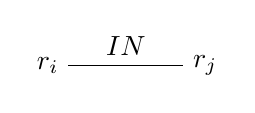
\begin{tikzpicture}
\node (ri) at (0,0) {$r_i$};
\node (rj) at (2,0) {$r_j$};
\draw (ri) to node[above,midway] {$IN$} (rj);
\end{tikzpicture}
\label{fig:subdigraphin}}
\subfigure[Input-output]{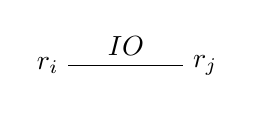
\begin{tikzpicture}
\node (ri) at (0,0) {$r_i$};
\node (rj) at (2,0) {$r_j$};
\draw (ri) to node[above,midway] {$IO$} (rj);
\end{tikzpicture}
\label{fig:subdigraphio}}
\caption{Subdigraphs in the i-dependency and io-dependency augmented digraph.}
\end{figure}


\begin{defi}[Rule having input-output dependency on another rule \wrtTx{} a set]
\term[Rule having input-output dependency on another rule \wrtTx{} a set]{Rule $r_i$ has an input-output dependency on rule $r_j$ \wrtTx{} a set $IO$}\tabbrev{Rule having input-output dependency on another rule \wrtTx{} a set}{IO-DEP} \iffTx{}
\begin{equation}
\fun{I}{\mbox{CHANGE}_i}\cap\fun{I}{\mbox{PRESET}_j}=\emptyset
\end{equation}
Where $IO=\accol{p|p\in\mbox{PRESET}_j\wedge\fun{I}{P}\cap\fun{I}{\mbox{CHANGE}_i}=\emptyset}$. If rule $r_i$ has an input-output dependency on rule $r_j$ \wrtTx{} the set $IO$, then in the io-dependency augmented digraph, there exists one subdigraph shown in figure \ref{fig:subdigraphio}.
\cite{conf/ijcai/HsuW89}
\end{defi}

\begin{defi}[Following rule set of a rule]
The \term{following rule set of a rule} $r$, \funm{Follow}{r}, is the set of all rules that are reachable from rule $r$ in the io-dependency augmented digraph unioned with the rule $r$ itself.
\cite{conf/ijcai/HsuW89}
\end{defi}

\begin{defi}[Descent rule of another rule]
If rule $r\in\funm{Follow}{r_i}$, then we call rule $r$ a \term{descent rule} of $r_i$.
\cite{conf/ijcai/HsuW89}
\end{defi}

\begin{defi}[Rule having an inference relation on another rule]
\term[Rule having an inference relation on another rule]{Rule $r_i$ has an inference relation on rule $r_j$} \tabbrev{Rule having an inference relation on another rule}{I-R} if there exists at least one rule $r\in\funm{Follow}{r_i}$ \stTx{} rule $r$ has an I-DEP on rule $r_j$ or rule $r_j$ has an I-DEP on rule $r$.
\cite{conf/ijcai/HsuW89}
\end{defi}

\begin{defi}[Derivation step, Derivation sequence]
Let $G_0$ be a set of object instantiations. We call $G_0\rightarrow^r G_1$ a \term{derivation step} if:
\begin{enumerate}
 \item for all $p\in\mbox{PRESET}_r$, if $p$ is marked $+$ and there exists one element $x$ of \fun{I}{p}, \stTx{} $x\in G_0$, or if $p$ is marked $-$, and \faTx{} $x$ in \fun{I}{p}, $x$ is not in $G_0$, and
 \item $G_1=G_0+\fun{A}{r}-\fun{D}{r}$ where \fun{A}{r} is the set of all object instances added by rule $r$, and \fun{D}{r} is the set of all object instances deleted by rule $r$. And let \fun{ILHS}{r} be the set of positive marked object instances, then \fun{D}{r} is a subset of \fun{ILHS}{r}.
\end{enumerate}
If $G_0\rightarrow^{r_1}G_1\rightarrow^{r_2}\ldots\rightarrow^{r_n}G_n$ we call $r_1\rightarrow r_2\rightarrow\ldots\rightarrow r_n$ a \term{derivation sequence}, which can be denoted by $r^{\star}$, then: $G_0\rightarrow^{r^{\star}}G_n$.
\cite{conf/ijcai/HsuW89}
\end{defi}

\begin{defi}[Equivalent derivation sequences]
Two derivation sequences $r_1^{\star}$ and $r_2^{\star}$ are called \term[Equivalent derivation sequences]{equivalent} if:
\begin{equation}
G_0\rightarrow^{r_1^{\star}}G_n\wedge G_0\rightarrow^{r_2^{\star}}G_m\wedge G_n=G_m
\end{equation}
The relation is denoted as $r_1^{\star}=r_2^{\star}$.
\cite{conf/ijcai/HsuW89}
\end{defi}
\chapter{Computer Vision and Pattern Recognition}

\chapter{Computer Science and Game Theory}

\begin{defi}
A \term{game} $A$ consists of the state of the \term{game objects} ($S$), the input of the system (player's input, $M$) and the abstract control system (time-independent, $F$) which governs the $S$ under the current $M$:
\begin{equation}
\mbox{Game }A=\tuple{S,M,F}
\end{equation}
\cite{journals/procedia/KosmadoudiLRSLSS12}
\end{defi}

\begin{defi}
\term{Neutral element} of $M$ (\term{empty input}, $\epsilon$) the current state of the game ($s$) with input ($p$) broken down into two consecutive inputs ($m$,$n$):
\begin{equation}
\group{
\fun{F}{s,\epsilon}=s\mbox{ with }s\in S\\
\fun{F}{s,mn}=\fun{F}{\fun{F}{s,m},n}\mbox{ with } s\in S\mbox{ and }m,n\in M
}
\end{equation}
\cite{journals/procedia/KosmadoudiLRSLSS12}
\end{defi}

\begin{defi}[Maxset, Minset]
The \term{maxset} $X^M$ is that subset of $X$ at which it is MAX's turn to make a move. The \term{minset} $X^m$ is that subset of $X$ at which it is MIN's turn to make a move.
\cite{conf/ijcai/Boffey73}
\end{defi}

\begin{defi}[Evaluation function, Better position]
An \termabbrev{evaluation function}{EF} over a game graph $\tuple{X,\Gamma}$ is a single valued function $\funsig{f}{X}{\RRR}$. If $\ffun{x}>\ffun{y}$ then $x$ is said to be a \term{better position} than $y$ under $f$.
\cite{conf/ijcai/Boffey73}
\end{defi}

\begin{defi}[Strategy $\calS_o$]
$\calS_o$ is that \term[Strategy $\calS_o$]{strategy} which leads to move $xy*$ being made from position $x$ where:
\begin{equation}
\group{\ffun{x*}=\displaystyle\max_{y\in\Gamma_x}\ffun{y}\mbox{ if }x\in X^M\\
\ffun{x*}=\displaystyle\min_{y\in\Gamma_x}\ffun{y}\mbox{ if }x\in X^m}
\end{equation}
Ties for $y*$ are broken by some subsidiary rule.
\cite{conf/ijcai/Boffey73}
\end{defi}

\begin{defi}[Locally equivalent evaluation functions, Locally perfect evaluation function]
Evaluation functions $f$ and $g$ are \term[locally equivalent evaluation functions]{locally equivalent} if
\begin{equation}
\ffun{x}>\ffun{y}\mbox{ whenever }\gfun{x}>\gfun{y}
\end{equation}
where $x,y\in\Gamma_w$ for some $w\in X$. $f$ is \term[locally perfect evaluation function]{locally perfect} if it is locally equivalent to $\lambda_{mm}^w$.
\cite{conf/ijcai/Boffey73}
\end{defi}

\begin{defi}[Probabilistic evaluation function]
A \termabbrev{probabilistic evaluation function}{PEF} over a game graph $\tuple{X,\Gamma}$ is a bounded function $\funsig{p}{X\times\RRR}{\RRR}$ with $\pfun{x,r}\geq0$, $\displaystyle\int{\pfun{x,r}\ dr}=1$ and $\pfun{x,r}=0$ outside some finite range $\fun{r_1}{x}\leq r\leq \fun{r_2}{x}$.
\cite{conf/ijcai/Boffey73}
\end{defi}

\begin{defi}[Strategy $\calS_o'$]
$\calS_o'$ is that \term[Strategy $\calS_o'$]{strategy} which leads to move $xy*$ being made from position $x$ where:
\begin{equation}
\group{\fun{v}{x*}_p=\displaystyle\max_{y\in\Gamma_x}\fun{v}{y}_p\mbox{ if }x\in X^M\\
\fun{v}{x*}_p=\displaystyle\min_{y\in\Gamma_x}\fun{v}{y}_p\mbox{ if }x\in X^m}
\end{equation}
\cite{conf/ijcai/Boffey73}
\end{defi}

\begin{defi}[(Constant) decision rule, Preference function, Preferred move]
A (constant) \termor{decision rule}{preference function} for MAX is a single valued function \funsig{\sigma_M}{X}{X} with $\fun{\sigma_M}{x}\in\Gamma_x$. $x\mapsto\fun{\sigma_M}{x}$ is MAX's \term{preferred move} from $x$. A preference function $\sigma_m$ for MIN can be defined in an analogous way.
\cite{conf/ijcai/Boffey73}
\end{defi}

\begin{defi}[(Constant) preference pair]
If $\sigma_M$ and $\sigma_m$ are preference functions for MAX and MIN respectively then $\sigma=\brak{\sigma_M,\sigma_m}$ is termed a (constant) \term{preference pair} on $\brak{X,\Gamma}$.
\cite{conf/ijcai/Boffey73}
\end{defi}

\begin{defi}[Strategy order relation $\leq_\sigma$]
If $u,v\in X$ and $\sigma$ is a preference pair on $\brak{X,\Gamma}$ then \term[Strategy order relation $\leq_\sigma$]{$u\geq_\sigma v$} \iffTx{} there exists an element $t\in X$ such that
\begin{enumerate}
 \item $u,v\in\Gamma^t$
 \item $u=\fun{\sigma_M}{t}$ or $v=\fun{\sigma_m}{t}$
\end{enumerate}
\cite{conf/ijcai/Boffey73}
\end{defi}

\begin{defi}[Evaluation function reproduces a preference pair]
An evaluation function $f$ over $\brak{X,\Gamma}$ \term[Evaluation function reproduces]{reproduces} a preference pair $\sigma$ (with respect to a strategy $\calS_0$) if $\ffun{x}>\ffun{y}$ whenever $x>_\sigma y$.
\cite{conf/ijcai/Boffey73}
\end{defi}

\begin{defi}[Strategy order relation $\leq_\sigma^*$]
If $u,v\in X$ and $\sigma$ is a preference pair on $\brak{X,\Gamma}$ then \term[Strategy order relation $\leq_\sigma^*$]{$u\geq_\sigma^* v$} \iffTx{} there exists is a sequence $u=w_0,w_1,\ldots,w_s=v$ such that $w_i>_\sigma w_{i-1}$, $i=1,2,\ldots,s$
\cite{conf/ijcai/Boffey73}
\end{defi}

\begin{defi}[Fully consistent strategy]
$\sigma$ is \term[Fully consistent strategy]{fully consistent} if $C_{\pi_1}=C_{\pi_2}$ for any pair of paths $\pi_1,\pi_2$ with the same endpoints.
\cite{conf/ijcai/Boffey73}
\end{defi}

\begin{defi}[(Variable) preference function]
A \term{(Variable) preference function} for MAX is a single-valued function \funsig{\tau_M}{X^M}{\Gamma\times X^M\setminus I} where $I$ is the unit interval $I=\accol{x|0\leq x\leq 1}$ and
\begin{enumerate}
 \item $\fun{\tau_M}{x,u}=0$ if $u\notin\Gamma_x$
 \item $\fun{\tau_M}{x,u}\geq 0$ if $u\in\Gamma_x$
 \item $\displaystyle\sum_{u\in\Gamma_x}{\fun{\tau_M}{x,u}}=1$
\end{enumerate}
\fun{\tau_M}{x,u} can be thought of as the probability that, when in position $x$, MAX will choose to move to position $u$. A variable preference rule $\tau_m$ for MIN can be defined in an analogous way.
\cite{conf/ijcai/Boffey73}
\end{defi}

\begin{defi}[(Variable) preference pair]
If $\tau_M$ and $\tau_m$ are variable preference functions for MAX and MIN respectively then $\tau=\brak{\tau_M,\tau_m}$ is termed a \term{(variable) preference pair} on \brak{X,\Gamma}.
\cite{conf/ijcai/Boffey73}
\end{defi}
\chapter{Machine Learning}

\begin{defi}[Learning algorithm for a meta-domain]%Problem: SxG??
Formally, an algorithm $A$ is a \term{learning algorithm for a meta-domain} $M$ in a hypothesis space $H$ with respect to a set of problem distributions $T$, if for any domain $D\in M$, any choice of a problem distribution $P$ in $T$, and any target problem solver $f\in H$,
\begin{enumerate}
\item $A$ takes as input the specification of a domain $D\in M$, an error parameter $E$, and a confidence parameter $\sigma$,
\item $A$ may call \alg{SolvedProblem}, which returns examples $\brak{x,\ffun{x}}$ for $D$, where $x$ is chosen with probability $\Pfun{x}$ from $S\times G$. The number of oracle calls of $A$ and its running time must be polynomial in the maximum problem size and the length of its input.
\item For all $D\in M$ and distributions $P\in T$, with probability at least $\brak{1-\delta}A$ outputs a program $f'$ that approximates $f$ in the sense that
\begin{equation}
\displaystyle\sum_{x\in\Delta}{\Pfun{x}}\leq\epsilon
\end{equation}
where $\Delta=\accol{x | f'\mbox{ fails on }x\mbox{ while }f\mbox{ succeeds}}$.
\item There is a polynomial $R$ such that, for a maximum problem size $n,\frac{1}{\epsilon},|frac{1}{\delta}$, maximum length $I$ and maximum step length $r$ of any solution output by \alg{SolvedProblem}, and an upper bound $t$ on the running times of programs in $D$ on inputs of size $n$, if $A$ outputs $f'$, the run time of $f'$ is bounded by $\fun{R}{n,l,r,t,\frac{1}{\epsilon},\frac{1}{\delta}}$
\end{enumerate}
\cite{conf/ijcai/Tadepalli91}
\end{defi}

\begin{defi}[Satisfying a spare solution space bias]
A problem solver $f$ for a domain $D$ and a problem distribution $P$ \term[Satisfying a sparse solution space bias]{satisfies a sparse solution space bias} if there is a set of operator sequences $m_f$ such that, on any problem $x\in D$ such that $\Pfun{x}>0$, $\ffun{x}\in m_f$ and $\abs{m_f}$ is bounded by a polynomial $Q$ in the problem size $n$.
\cite{conf/ijcai/Tadepalli91}
\end{defi}

\begin{defi}[Satisfying a macro table bias]
A problem solver $f$ \term[Satisfying a macro table bias]{satisfies a macro table bias} for a domain $D$ in $M$ if there is a feature ordering $O=\brak{l,\ldots,n}$ such that,
\begin{enumerate}
 \item $D$ is serially decomposable for $O$, and
 \item $f$ constructs all its solutions using a macro table $M$ as follows: for each feature $i$ from $1$ to $n$, macros $M_{j,i}$ are successively applied, where $j$ is the value of feature $i$ in the state before applying the macro.
\end{enumerate}
\cite{conf/ijcai/Tadepalli91}
\end{defi}

\begin{defi}[Beliefs in Conjoint Analysis]
We allow weighted beliefs with a weight parameter coming from \ocinterval{0}{1} where $1$ means full truth degree (complete certainty, the perfect belief), while a value $\alpha\in\oointerval{0}{1}$ describe a regular belief that can be doubted.
\begin{enumerate}
 \item \term{Regular belief}s such as:
 \begin{equation}
(\fun{A_1}{a_1}\wedge\ldots\wedge\fun{A_t}{a_t}):\alpha
 \end{equation}
 \item \term{Indifference belief}s such as:
 \begin{equation}
 \left(L\leftrightarrow R\right):1
 \end{equation}
 Indifference beliefs are always have full truth because we claim that if the respondent would distinguish degrees of truth then she is able to express preference.
 \item \term{Negative belief}s such as:
 \begin{equation}
 \left(\neg F\right):1
 \end{equation}
\end{enumerate}
where $A_i$ are attribute predicates and $L$, $R$, $F$ are regular atom conjunctions. Again, it is obvious in conjoint to don't ask user to express thoughts on negative information. As such there are no real negative beliefs such as $F:0$. Moreover, the reader may notice that we adopt the intuitionistic logic approach i.e., there is no assumption on any kind of law of excluded middle, as we don't necessarily assume $F:0\Leftrightarrow\left(\neg F\right):1$.
\cite{conf/fedcsis/GiurcaSB12}
\end{defi}

\begin{defi}[Single-controller-stochastic-game, stage game, agent, adversary, probabilistic transition function]
A \termabbrev{single-controller-stochastic-game}{SCSG} $M$ on states $S=\accol{1,2,\ldots,N}$ and actions $A=\accol{a_1,a_2,\ldots,a_k}$, consists of:
\begin{enumerate}
 \item \term[Stage game]{Stage games}: each state $s\in S$ is associated with a zero-sum game in strategic form, where the action set of each player is $A$. The first player is termed \term{agent} and the second player is termed \term{adversary}.
 \item \term{Probabilistic transition function}: $\fun{P_M}{s,t,a}$ is the probability of a transition from $s$ to $t$ given that the first player (termed agent), plays $a$.
\end{enumerate}
\cite{Brafman:1999:NPA:1624312.1624324}
\end{defi}

\begin{defi}[$\alpha$-approximation of a single-controller-stochastic-game]
Let $M$ and $\overline{M}$ be single-controller-stochastic-games over the same state space. We say that $\overline{M}$ is an \term[$\alpha$-approximation of a single-controller-stochastic-game]{$\alpha$-approximation of $M$} if for every state $s$ we have:
\begin{enumerate}
 \item If \fun{P_M}{s,t,a} and \fun{P_{\overline{M}}}{s,t,a} are the probabilities of transition to $t$ given that the action carried out by the agent is $a$, in $M$ and $\overline{M}$ respectively, then, $\fun{P_M}{s,t,a}-\alpha\leq \fun{P_{\overline{M}}}{s,t,a}\leq \fun{P_M}{s,t,a}+\alpha$
 \item The game associated with $s$ in $\overline{M}$ is the game associated with it in $M$ restricted to a non-empty subset of the columns.
\end{enumerate}
\cite{Brafman:1999:NPA:1624312.1624324}
\end{defi}

\begin{defi}[Induced single-controller-stochastic-game]
Let $M$ be an single-controller-stochastic-game, and let $L$ be any subset of $S$. The \term{induced single-controller-stochastic-game}, $M_L$ , has states $L\cup\accol{l_0}$, and transitions and state games as follows:
\begin{enumerate}
 \item The states in $M_L$ are associated with the same games as in $M$.
 \item The state $l_0$ is associated with a game where the adversary obtains the value $P_{\mbox{max}}$ for any joint action (a "worst case" state for the agent).
 \item For any action $a,\fun{P_{M_L}}{l_0,l_0,a_0}=1$.
 \item For any states $s,t\in L$, and $a\in A$, we have that $\fun{P_M}{s,t,a}=\fun{P_{M_L}}{s,t,a}$.
 \item For every $s\in L$, and $t\notin L$, and for every action $a\in A$, we have that $\fun{P_{M_L}}{s,t,a}=0$.
 \item For every $s\in L$, and $a\in A$, we have that $\fun{P_{M_L}}{s,l_0,a}=\displaystyle\sum_{j\notin L}{\fun{P_M}{s,t,a}}$.
\end{enumerate}
\cite{Brafman:1999:NPA:1624312.1624324}
\end{defi}


\section{Empirical Law Discovery}

\begin{defi}[$X$-of-$N$ representation]
Let \accol{A_i|1\leq i\leq\mbox{MaxAtt}} be the set of attributes of a domain, and for each $A_i$, \accol{V_{ij}|1\leq j\leq\mbox{MaxAttVal}_i} be its value set where $\mbox{MaxAtt}$ is the number of attributes, and $\mbox{MaxAttVal}_i$, is the number of different values of $A_i$. An \term{$X$-of-$N$ representation} is a set, denoted as $\mbox{$X$-of-}\accol{AV_k|AV_k\mbox{ is an attribute-value pair denoted as ``}A_i=V_{i,j}\mbox{'', }1\leq k\leq N_+, N\leq N_+, 1\leq N\leq\mbox{MaxAtt}}$, where $N_+$ is the number of attribute-value pairs in the $X$-of-$N$ representation, called the size of the $X$-of-$N$ representation, and $N$ is the number of different attributes that appear in the $X$-of-$N$ representation. The value of an $X$-of-$N$ can be any number between $0$ and $N$. Given an instance, its value is $X$ \iffTx{} $X$ of the $AV_k$ are true. An attribute-value pair $\fun{AV_k}{A_i=V_{ij}}$ is true for an instance \iffTx{} attribute $A_i$, of the instance has value $V_{ij}$.
\cite{conf/ijcai/Zheng95}
\end{defi}

\section{Reinforcement Learning}

\begin{defi}[$\mu$-approximation $T$-step planning algorithm for a Dynamic Bayesian Network-Markov Decision Processes]
A \term{$\mu$-approximation $T$-step planning algorithm for a Dynamic Bayesian Network-Markov Decision Processes} is one that, given a Dynamic Bayesian Network-Markov Decision Processes, produces a (compactly represented) policy n such that $\fun{U_M^{\pi}}{x,T}\geq\brak{1-\mu}\fun{U_M^{\star}}{x,T}$.
\cite{conf/ijcai/KearnsK99}
\end{defi}

\begin{defi}[induced Dynamic Bayesian Network-Markov Decision Processes on a subset of the transition components of a Dynamic Bayesian Network-Markov Decision Processes]
Let $M$ be a Dynamic Bayesian Network-Markov Decision Processes and let $T$ be any subset of the transition components in the model. The \term[induced Dynamic Bayesian Network-Markov Decision Processes on a subset of the transition components of a Dynamic Bayesian Network-Markov Decision Processes]{induced Dynamic Bayesian Network-Markov Decision Processes on $T$}, denoted $M_T$, is defined as follows:
\begin{enumerate}
 \item $M_T$ has the same set of sate variables as $M$; however in $M_T$ each variable $X_i$ has, in addition to its original set of values \fun{\mbox{Val}^M}{X_i}, a new value $w$.
 \item $M_T$ has the same transition graphs as $M$. For each $a$, $i$ and $u\in\fun{\mbox{Val}^M}{\fun{\mbox{Pa}_a}{X'_i}}$, we have that $\fun{P_a^{M_T}}{X_i'|u}=\fun{P_a^M}{X_i'|u}$ if the corresponding transition component is in $T$; in all other cases, $\fun{P_a^{M_T}}{w|u}=1$ and $\fun{P_a^{M_T}}{x_i|u}=0$ for all $x_i\in\fun{\mbox{Val}^M}{X_i}$.
 \item $M_T$ has the same set $\calR$ as $M$. For each $i=1,2,\ldots,k$ and $c\in\fun{\mbox{Val}^M}{C_i}$, we have that $\fun{R_i^{M_T}}{c}=\fun{R_i^M}{c}$. For other vectors $c$, we have that $\fun{R_i^{M_T}}{c}=-R_{\mbox{max}}$.
\end{enumerate}
\cite{conf/ijcai/KearnsK99}
\end{defi}

\begin{defi}[$\epsilon$-mixed Markov chain at a certain moment in time]
Let $Q$ be a transition model for a Markov chain and let $\accol{X^{\brak{t}}}_{t=0}^{\infty}$ represent the state of the chain. Let $S=\accol{x_1,x_2,\ldots,x_s}$. Let $\mu_j$ be the stationary probability of $x_j$ in the Markov chain. We say that Markov chain $Q$ is \term[$\epsilon$-mixed Markov chain at a certain moment in time]{$\epsilon$-mixed at time $m$} if $\max_{i,j}\abs{\fun{P}{X^{\brak{t}}=x_j|X^{\brak{1}}=x_i}-\mu_j}\leq\epsilon$.
\cite{conf/ijcai/KearnsK99}
\end{defi}

\begin{defi}[Dependency graph for the Dynamic Bayesian Network]
Consider a Dynamic Bayesian Network over the state variables $X_1,X_2,\ldots,X_n$ .The \term[Dependency graph for the Dynamic Bayesian Network]{dependency graph $V$ for the Dynamic Bayesian Network} is a directed cyclic graph whose nodes are $X_1,X_2,\ldots,X_n$ and where there is a directed edge from $X_i$ to $X_j$ if there is an edge in the transition graph of the Dynamic Bayesian Network from $X_i'$ to $X_j'$.
\cite{conf/ijcai/KearnsK99}
\end{defi}
\chapter{Logic in Computer Science}

\section{First-Order Logic}

\begin{defi}[Signature]
$S$ is a \term{signature} if $S$ is a four-tuple \tuple{P,F,r,C} where:
\begin{enumerate}
\item $P$ is a set of \term{predicate symbols} \brak{P_1,P_2,\ldots,P_n},
\item $F$ is a set of \term{function symbols} \brak{F_1,F_2,\ldots,F_m},
\item $r$ is \term{arity} or \term{degree of functions} and relations. For each $P_i$ respectively $F_j$, \fun{r}{P_i} respectively \fun{r}{F_j} is a non-zero natural number denoting the arity of $P_i$ respectively $F_j$,
\item $C$ is a set of \term{constant symbols}.
\end{enumerate}
\cite{conf/fedcsis/Telnarova12}
\end{defi}

\begin{defi}[Alphabet]
An \term{alphabet} $\Sigma$ consists of the following symbols:
\begin{enumerate}
\item Signature $S=\tuple{P,F,r,C}$.
\item \term{Collection of variables} $V$.
\item \term{Operators}: $\neg$ (\term{negation}), $\wedge$ (\term{conjunction}), $\vee$ (\term{disjunction}), $\rightarrow$ (\term{implication}), $\leftrightarrow$ (\term{equivalence}).
\item \term{Quantifiers}: $\forall$ (\term{forall}), $\exists$ (\term{exists}).
\item \term{Parentheses} and \term{punctuation symbols}: $($, $)$ and $,$.
\end{enumerate}
\cite{conf/fedcsis/Telnarova12}
\end{defi}

\begin{defi}[Term]
A \term{term} is defined inductively as follows:
\begin{enumerate}
\item Variable is term.
\item Constant is term.
\item If $f$ is a function symbol ($f\in F$) with arity $m$ and $t_1,t_2,\ldots,t_m$ are terms of $\Sigma$, then \ffun{t_1,t_2,\ldots,t_m} is term of $\Sigma$.
\end{enumerate}
\cite{conf/fedcsis/Telnarova12}
\end{defi}

\begin{defi}[Atom]
If $p$ is predicate symbol with arity $m$ and $t_1,t_2,\ldots,t_m$ are terms of $\Sigma$, then $\fun{p}{t_1,t_2,\ldots,t_m}$ is an \termor{atomic formula}{atom}. An atomic formula is a \term{formula} and all occurrences of variables in an atomic formula are free.
\cite{conf/fedcsis/Telnarova12}
\end{defi}

\begin{defi}[Formula]
A \term{formula} is defined as follows:
\begin{enumerate}
 \item An atom is a formula.
 \item If $H$ and $G$ are formulas, then:
 \begin{enumerate}
  \item $\neg H$ is a formula, the occurrence of variables in $\neg H$ is free respectively bound if it is free respectively bound in $H$,
  \item $H\wedge G$ is a formula, the occurrence of variables in $H\wedge G$ is free respectively bound if it is free respectively bound in $H$ or $G$,
  \item $H\vee G$ is a formula, the occurrence of variables in $H\vee G$ is free respectively bound if it is free respectively bound in $H$ or $G$,
  \item $H\rightarrow G$ is a formula, the occurrence of variables in $H\rightarrow G$ is free respectively bound if it is free respectively bound in $H$ or $G$,
  \item $H\leftrightarrow G$ is a formula, the occurrence of variables in $H\leftrightarrow G$ is free respectively bound if it is free respectively bound in $H$ or $G$.
 \end{enumerate}
 \item If $H$ is a formula and $x$ is a variable, then $\forall x:H$ and $\exists x:H$ are formulas. All occurrences of $x$ are bound.
\end{enumerate}
\cite{conf/fedcsis/Telnarova12}
\end{defi}

\begin{defi}[Literal]
A \term{literal} $L$ is an atom or the negation of an atom.
\cite{conf/fedcsis/Telnarova12}
\end{defi}

\begin{defi}[Clause]
A \term{clause} is a formula such as $\forall\vec{x}:L_1\vee L_2\vee\ldots\vee L_m$ where each $L_i$ is a literal and $\vec{x}=\brak{x_1,x_2,\ldots,x_n}$ are all the variables occurring in $L_1\vee L_2\vee\ldots\vee L_m$.
\cite{conf/fedcsis/Telnarova12}
\end{defi}

\begin{defi}[Horn-clauses]
\term{Horn-clause}s have the form: $\forall x_1,x_2,\ldots,x_n:L_1\wedge L_2\wedge\ldots\wedge L_m\rightarrow L$ where $L,L_1\wedge L_2\wedge\ldots\wedge L_m$ are a literals and $x_1,x_2,\ldots,x_n$ are all variables having free occurrences in $L,L_1\wedge L_2\wedge\ldots\wedge L_m$.
\cite{conf/fedcsis/Telnarova12}
\end{defi}

\begin{defi}[Negation of a dilemma, Conjunction of dilemmas, Disjunction of dilemmas]
For a given set $D$ of dilemmas it is defined:
\begin{enumerate}
 \item A \term{negation of a dilemma} $d=\dilemma{u}$ as a dilemma $\neg d=\negdilemma{u}$;
 \item A \term{disjunction of the dilemmas} $d'=\dilemma{u'}$, $d''=\dilemma{u''}$ as a dilemma $d'\vee d''=\flatbrak{u'\vee u''|\neg\brak{u'\vee u''}}$;%
 \item A \term{conjunction of the dilemmas} $d'=\dilemma{u'}$, $d''=\dilemma{u''}$ as a dilemma $d'\wedge d''=\flatbrak{u'\wedge u''|\neg\brak{u'\wedge u''}}$;%
\end{enumerate}
\cite{conf/fedcsis/Kulikowski12}
\end{defi}

\begin{defi}[Equal certainty relation, Ambivalent dilemma, Equivalent dilemmas, Anti-equivalent dilemmas]
Let $D$ be a set of dilemmas. Then in $D$ a binary relation $\approx^c$ satisfying the conditions of:
\begin{enumerate}
\item Reciprocity: for each $d\in D$ it holds $d\approx^c d$;
\item Symmetry: for any $d',d''\in D$ if $d'\approx^c d''$ then also $d''\approx^c d'$ holds;
\item Reflexivity: for any $d',d''\in D$ if $d'\approx^c d''$ then also $\neg d'\approx^c\neg d''$ holds;
\item Transitivity: for any $d',d'',d'''\in D$ if $d'\approx^c d''$ and $d''\approx^c d'''$ then also $d'\approx^c d'''$ holds;
\item Fixation: for any $d',d''\in D$ if $d'\approx^c\neg d'$ and $d''\approx^c\neg d''$ then also $d'\approx^c d''$ holds,
\end{enumerate}
will be called an \term{equal certainty relation}. Any dilemma satisfying the condition $d\approx^c\neg d$ will be called an \term{ambivalent dilemma}; any dilemmas such that $d'\approx^c d''$ holds will be called \term{equivalent dilemmas}; any dilemmas such that $d'\approx^c\neg d''$ holds will be called \term{anti-equivalent dilemmas}.
\cite{conf/fedcsis/Kulikowski12}
\end{defi}

\begin{defi}[Certainty ranking]
Let $D$ be a set of dilemmas with established equal certainty relation. Then a binary relation $\preceq^c$ described in $D$ and satisfying the conditions of:
\begin{enumerate}
 \item reciprocity: for each $d\in D$ it holds $d\preceq^c d$;
 \item symmetry: for any $d',d''\in D$ $d'\preceq^c d''$ and $d''\preceq^c d'$ hold if and only if $d'\approx^c d''$ holds;
 \item anti-reflexivity: for any $d',d''\in D$ if $d'\preceq^c d''$ then $\neg d''\preceq^c\neg d'$ holds;
 \item transitivity: for any $d',d'',d'''\in D$ if $d'\preceq^c d''$ and $d''\preceq^c d'''$ then also $d'\preceq^c d'''$ holds,
\end{enumerate}
will be called a \term{certainty ranking}.
\cite{conf/fedcsis/Kulikowski12}
\end{defi}

\begin{theo}
Let $D$ be a set of dilemmas with established equal certainty and certainty ranking relations. Then for any $d',d''\in D$:
\begin{enumerate}
\item if $d'\preceq^c d''$ and not $d''\preceq^c d'$ then $d'\vee d''\preceq^c d''$;
\item if $d'\preceq^c d''$ and not $d''\preceq^c d'$ then $d'\wedge d''\preceq^c d'$;
\item if $d'\approx^c d''$ then $d'\vee d''\approx^c d'\wedge d''\approx^c d'\approx^c d''$;
\item if $d'\approx^c d''$ then $d'\wedge d''\approx^c d',d''$;
\item if $d'\approx^c d''$ then $d',d''\approx^c d'\vee d''$
\end{enumerate}
\cite{conf/fedcsis/Kulikowski12}
\end{theo}

\section{Logic Programming}

\begin{defi}[Domain declaration for predicate symbol $p$]
A \term{domain declaration for predicate symbol $p$} of arity n is an expression of the following form.
\begin{equation}
\mbox{domain }\fun{p}{a_1,\ldots ,a_n}
\end{equation}
where $a_i$ is either $h$ or $d$. When $a$ is equal to $h$, this means that the $i$-th argument of $p$ ranges over the Herbrand universe. Otherwise, it means that the $i$-th argument is a list of variables which ranges over $d_1$ In the following, the domains $d_i$ are finite and explicit sets of values (i.e constants).
\cite{conf/ijcai/Hentenryck87}
\end{defi}

\begin{defi}[Domain set of a logic program]
Let $dl,\ldots ,dn$ the domains appearing in the domain declarations of a logic program $PR$ and different from the Herbrand universe. We note \fun{D}{PR} the set $\accol{d|d\neq\emptyset\wedge d\in 2^{d_i}\accol{1\leq i\leq n}}$ We call it the \term{domain set of the logic program}. The domain set of a logic program contains all domains we possibly need during the computations.
\cite{conf/ijcai/Hentenryck87}
\end{defi}

\begin{defi}[Range of a term included in a domain]
We say that the \term{range of $t$ is included in a domain $d_t$} denoted $\abs{t}\in d_i$ if $t$ is a constant $\in d_t$ or a $d$-variable $x^{d_t}$ such that $d_t\subseteq d$
\cite{conf/ijcai/Hentenryck87}
\end{defi}

\begin{defi}[$d$-substitution]
A $d$-substitution $\theta$ is a finite set of the form $\accol{v_1/t_1,\ldots,v_n/t_n}$ where
\begin{enumerate}
 \item each $v_i$ is either a variable or $d$-variable
 \item $t_i$ is a term distinct from $v_i$,
 \item $v_1,\ldots,v_n$ are all distinct,
 \item if $v_i$ is a $d$-variable $v^{d_i}$, $\abs{t_i}\in d_i$
\end{enumerate}
\cite{conf/ijcai/Hentenryck87}
\end{defi}

\begin{defi}[$d$-substitutions agree on a set of variables and $d$-variables]
We say that two \term[$d$-substitutions agree on a set of variables and $d$-variables]{$d$-substitutions $\theta$ and $\lambda$ agree on a set $V$ of variables and $d$-variables}, denoted $\theta=\lambda\abs{V}$ \iffTx{} $x\theta=x\lambda$ for each $x\in V$ where $=$ denotes syntactic equality.
\cite{conf/ijcai/Hentenryck87}
\end{defi}

\begin{defi}[$d$-instance]
$\theta$ is a \term{$d$-instance} of $\lambda$ in $V$, denoted $\lambda\leq\theta$ \iffTx{} $x\theta=\delta\circ\lambda$ for some $d$-substitution $\delta$.
\cite{conf/ijcai/Hentenryck87}
\end{defi}

\begin{defi}[$d$-unifier, unifies, more general $d$-unifier, $d$-mgu]
A $d$-substitution $\sigma$ is a \term{$d$-unifier} of some non-empty and finite subset $S=\accol{t_1,\ldots,t_n}$ where $t_i$ and a literal of a term \iffTx{} $t_1\sigma=\ldots=t_n\sigma$, we also say that $\sigma$ \term{unifies} $S$. \term{\fun{UNI}{S}} is the set of all $d$-unifiers of $S$. $\sigma$ is called the \termor{more general $d$-unifier}{$d$-mgu} of $S$ \iffTx for each $\theta\in\fun{UNI}{S}$, $\theta\leq\sigma\abs{\fun{vars}{S}}$ implies $\sigma\leq\theta\abs{\fun{vars}{S}}$ where \fun{vars}{S} is the set of all variable or $d$-variable symbols in $S$.
\cite{conf/ijcai/Hentenryck87}
\end{defi}

\begin{defi}[Constraint]
Let $p$ be a $n$-ary predicate symbol, $p$ is a \term{constraint} \iffTx for any ground terms either has a successful refutation or has only finitely failed derivations.
\cite{conf/ijcai/Hentenryck87}
\end{defi}

\begin{defi}[forward checkable literal, forward-variable]
A literal $\pfun{x_1,\ldots,x_n}$ in the resolvent is \term[forward checkable literal]{forward checkable} \iffTx{} $p$ is a constraint and all it's arguments are ground but one which is a $d$-variable. This $d$-variable is called the \term{forward-variable}.
\cite{conf/ijcai/Hentenryck87}
\end{defi}

\begin{defi}[forward checking inference rule]
Let $G_1$ be the goal $\leftarrow A_1,\ldots,A_{m-1},P,A_{m+1},\ldots A_k$ and $PR$ be a logic program. $G_{i+1}$ is derived from $G_i$ using the mgu $\theta_{i+1}$ via $PR$ if the following conditions hold:
\begin{enumerate}
 \item $P$ is forward checkable and $x^d$ is the forward variable
 \item $d_{\mbox{new}}=\accol{a\in d|PR\vDash P\accol{x/a}}$ and $d_{\mbox{new}}\neq\emptyset$
 \item $\theta_{i+1}$ is
 \begin{enumerate}
  \item $\accol{x^d/e}$ if $d_{\mbox{new}}=\accol{e}$
  \item $\accol{x^d/z^{d_{\mbox{new}}}}$ where $z^d_{\mbox{new}}$ is a new variable otherwise.
 \end{enumerate}
 \item $G_{i+1}$ is the goal $\leftarrow\brak{A_1,\ldots,A_{m-1},A_{m+1},\ldots A_k}\theta_{i+1}$
\end{enumerate}
Such a derivation rule is called the \termabbrev{forward checking inference rule}{FCIR}.
\cite{conf/ijcai/Hentenryck87}
\end{defi}

\begin{defi}[Efficient computation rule with respect to forward declarations]
A computation rule is \term[Efficient computation rule with respect to forward declarations]{efficient with respect to the forward declarations}, if it selects only a predicate submitted to forward declaration when it is ground or forward checkable and if, whenever the resolvent contains literals submitted to a forward declaration which are either forward-checkable or ground, it selects one of them.
\cite{conf/ijcai/Hentenryck87}
\end{defi}

\begin{defi}[lookahead checkable literal, lookahead-variable]
A literal $\pfun{t_1,\ldots,t_n}$ in the resolvent is \term[lookahead checkable literal]{lookahead checkable} \iffTx{} $p$ is a constraint and their exists at least one $t_i$ which is a domain-variable and each other argument is either ground or a domain-variable. The domain-variables in $t_1,\ldots,t_n$ are called the \term{lookahead-variable}s.
\cite{conf/ijcai/Hentenryck87}
\end{defi}

\begin{defi}[lookahead inference rule]
Let $G_1$ be the goal $\leftarrow A_1,\ldots,A_{m-1},P,A_{m+1},\ldots A_k$ and $PR$ be a logic program. $G_{i+1}$ is derived from $G_i$ using the mgu $\theta_{i+1}$ via $PR$ if the following conditions hold:
\begin{enumerate}
 \item $P$ is lookahead checkable and $x_1,\ldots,x_n$ are the lookahead variables whose domains are $d_{x_1},\ldots d_{x_n}$.
 \item For each $x_j^{d_{x_j}}$ let:
 \begin{enumerate}
  \item $d_{z_j}=\accol{y_j\in d_{x_j}|\exists y_1\in d_{x_1},\ldots,y_{j-1}\in d_{x_{j-1}},y_{j+1}\in d_{x_{j+1}},\ldots,y_n\in d_{x_n}\mbox{ such that }PR\vDash P\theta\mbox{ with }\theta=\accol{x_1/y_1,\ldots,x_n/y_n}}$ and $d_{x_j}\neq\emptyset$.
  \item $e_j$ as
  \begin{enumerate}
   \item a new variable of domain $d_{z_j}$ if $d_{z_j}=\abs{\accol{e_1,\ldots,e_l}}>1$.
   \item the constant $e$ if $d_{z_j}$ if $d_{z_j}=\accol{e}$.
  \end{enumerate}
 \end{enumerate}
 \item $\theta_{i+1}=\accol{x_1/z_1,\ldots,x_n/z_n}$
 \item $G_{i+1}$ is the goal
 \begin{enumerate}
  \item $\leftarrow\brak{A_1,\ldots,A_{m-1},A_{m+1},\ldots A_k}\theta_{i+1}$ if at most one $z_i$ is a $d$-variable.
  \item $\leftarrow\brak{A_1,\ldots,A_{m-1},P,A_{m+1},\ldots A_k}\theta_{i+1}$ otherwise.
 \end{enumerate}
\end{enumerate}
Such a derivation rule is called the \termabbrev{lookahead inference rule}{LAIR}.
\cite{conf/ijcai/Hentenryck87}
\end{defi}

\begin{defi}[Efficient computation rule with respect to the lookahead declarations]
A computation rule is \term[efficient computation rule with respect to the lookahead declarations]{efficient with respect to the lookahead declarations}, if a literal in the resolvent submitted to a lookahead declaration is only selected if either it is lookahead checkable or all its arguments are ground.
\cite{conf/ijcai/Hentenryck87}
\end{defi}

\begin{defi}[\fun{Revise}{M,a}]
Let $a$ be a formula and M a model. \term{\fun{Revise}{M,a}} is the set of models $M'$ such that
\begin{enumerate}
\item \label{reviseIt1} $M'$ and $M$ have the same universe and agree on all functions.
\item \label{reviseIt2} $a$ and the protected formulas of $T$ are true in $M'$.
\item There is no other model $M''$ such that for some $1<i<1$,
\begin{enumerate}
\item $M''$ satisfies (\ref{reviseIt1}) and (\ref{reviseIt2});
\item $M''$ and $M'$. agree on all predicates in strata $1$ through $i-1$; and
\item the differences between M" and M on predicates in stratum $i$ are a proper subset of the differences between $M'$ and $M$ on those predicates.
\end{enumerate}
\end{enumerate}
\cite{conf/ijcai/Winslett89}
\end{defi}

\begin{defi}[Preferred model at the $i$-th stratum]
A model $\calM_1$ is \term[Preferred model at the $i$-th stratum]{preferred to model $\calM_2$ at the $i$-th stratum} (written $\calM_1<_i\calM_2$) \iffTx{}
\begin{enumerate}
\item $\calM_1$ and $\calM_2$ have identical universes;
\item $\calM_1$ and $\calM_2$ agree on all predicates and functions, except possibly those of $S_i$ and $V_i$;
\item For all predicates $P$ in stratum $S_t$, and for all $\bar{x}$ such that $\fun{P}{\bar{x}}$ is true in $\calM_1$, $\fun{P}{\bar{x}}$ is true in $\calM_2$; and
\item For some predicate $P$ in stratum $S_i$ and some $\bar{x}$, $\fun{P}{\bar{x}}$ is false in $\calM_1$ and true in $\calM_2$.
\end{enumerate}
\cite{conf/ijcai/Winslett89}
\end{defi}

\begin{defi}[Abductive problem, Background theory of the abductive problem, Abducible set of the abductive problem, Goal of the abductive problem, Solution of an abductive problem, Minimal solution of an abductive problem]
The triple $\tuple{\Pi,A,g}$ is an \term{abductive problem} \iffTx{} $\Pi$ is a set of propositional Horn Clauses (called the \term{background theory of the abductive problem}), $A$ a set of propositions (called the \term{abducible set of the abductive problem}) and $g$ is a proposition (called the \term{goal of the abductive problem}). The set of propositions $\Delta$ is a \term[solution of an abductive problem]{solution of the abductive problem} $\tuple{\Pi,A,g}$ \iffTx{}
\begin{enumerate}
\item $\Delta\subseteq A$
\item $\Delta\cup\Pi\vdash g$
\item $\Delta\cup\Pi$ is consistent
\item $\brak{a\in A \wedge \Delta+\Pi\vdash a}\rightarrow a\in\Delta$
\end{enumerate}
$\Delta$ is a \term[Minimal solution of an abductive problem]{minimal solution of} $\tuple{\Pi,A,g}$ \iffTx{} it is a solution of $\tuple{\Pi,A,g}$ and no subset of $\Delta$ is a solution of $\tuple{\Pi,A,g}$.
\cite{conf/ijcai/Eshghi93}
\end{defi}

\begin{defi}[Only-if set, \fun{only-if}{T,S}, \fun{only-if}{T}, \fun{props}{T}]
Let the clauses $p\leftarrow Q_1,p\leftarrow Q_2,\ldots,p\leftarrow Q_k$. where $Q_1,Q_2,\ldots,O_k$ are conjunctions of propositions, be all the clauses in $\Pi$ which have $p$ at their head. Let $n_{c_1},n_{c_2},...,n_{c_k}$ be the names of these clauses. Then the \term{only-if set} of p with respect to $\Pi$ is $\accol{\neg p\vee n_{c_1}\vee n_{c_2}\vee\ldots\vee n_{c_k},n_{c_1}\rightarrow Q_1,n_{c_2}\rightarrow Q_2,\ldots,n_{c_k}\rightarrow Q_k}$. For at set of propositions $S$ and the Horn clause theory $T$, we use \term{\fun{only-if}{T,S}} to denote the union of only-if sets of all the propositions in $S$ with respect to $T$. We use \term{\fun{only-if}{T}} to denote \fun{only-if}{T,\fun{props}{T}} where \term{\fun{props}{T}} is the set of all propositions in $T$.
\cite{conf/ijcai/Eshghi93}
\end{defi}

\begin{defi}[Truth-assignment, Model]
Let $C$ be a propositional clausal theory. $S$ the set of propositions in $C$, and $M$ a set of propositions. Then the \term{truth-assignment} induced by $M$ is the assignment of true to all propositions in $S$ which are in $M$. and false to those propositions in $S$ which are not in $M$. $M$ is a \term{model} of $C$ \iffTx{} the truth assignment induced by $M$ satisfies all the clauses in $C$.
\cite{conf/ijcai/Eshghi93}
\end{defi}

\begin{defi}[Model which minimizes, Minimization with respect to]
Let $C$ be a propositional clausal theory. and $A$ a set of propositions. Then $M$ is a \term[model which minimizes]{model of $C$ which minimizes $A$} \iffTx{}
\begin{enumerate}
 \item $M$ is a model of $C$
 \item There is no other model $M'$ of $C$ such that $M'\cap A\subseteq M\cap A$
\end{enumerate}
We say that $\Delta$ is a \term[minimization with respect to]{minimization of $A$ with respect to $C$} \iffTx{} there is a model $M$ of $C$ which minimizes $A$ and $\Delta=M\cap A$
\cite{conf/ijcai/Eshghi93}
\end{defi}

\begin{defi}[Unit refutable]
A propositional clausal theory $C$ is \term{unit refutable} \iffTx{}, for every set of unit clauses $U$, if $C\cup U$ is inconsistent. then the empty clause is unit-derivable from $C\cup U$.
\cite{conf/ijcai/Eshghi93}
\end{defi}

\begin{defi}[Connection graph]
Given a set of clauses $C$. the \term{connection graph} of $C$ is the graph obtained by drawing a link between each complimentary pair of literals in the set.
\cite{conf/ijcai/Eshghi93}
\end{defi}

\begin{defi}[Chain]
Given the set of clauses $C$, the sequence $\flatbrak{\brak{x_1,e_1,y_1},\brak{x_2,e_2,y_2},\ldots,\brak{x_n,e_n,y_n}}$ of $c$-triples is a \term{chain} in $C$ \iffTx{} for all $k$, $e_k$ is a clause in $C$ and $y_k=\neg x_{k+1}$.
\cite{conf/ijcai/Eshghi93}
\end{defi}

\begin{defi}[Tied chain]
$\flatbrak{\brak{x_1,e_1,y_1},\brak{x_2,e_2,y_2},\ldots,\brak{x_n,e_n,y_n}}$ is a \term{tied chain} in $C$ \iffTx{} it is a chain in $C$ and $x_1=y_n$.
\cite{conf/ijcai/Eshghi93}
\end{defi}

\begin{defi}[Subgoal clause]
Let $C$ be a set of clauses. Let $T$ be a connection tableau for $C$. Let $s_1,s_2,\ldots,s_n$, $n\geq 1$ be the subgoals of $T$ Then we call $s_1\vee s_2\vee\ldots\vee s_n$ the \term{subgoal} clause of $T$.
\cite{conf/ijcai/Fuchs99}
\end{defi}

\begin{defi}[Query tableau, Query clause]
Let $\calC$ be a set of clauses. Let $T$ be a connection tableau for $\calC$. Let $\calS\subseteq \calC$ be a set of start clauses. Let $S$ be the clause below the unlabeled root of $T$. If $S$ is an instance of a clause from $\calS$ we call$T$ a \term{query tableau} (\wrtTx{} $\calS$) and the subgoal clause of $T$ a \term{query clause} (\wrtTx{} $S$).
\cite{conf/ijcai/Fuchs99}
\end{defi}

\begin{defi}[Lemma tableau, Lemma clause]
Let $\calC$ be a clause set. Let $T$ be a connection tableau for $\calC$. Let $C=s_1\vee s_2\vee\ldots\vee s_n$ be the subgoal clause of $T$. Let $\calH$ be the set of subgoals which are immediate successors of the root. If $\calH\neq\emptyset$ we call $T$ a \term{lemma tableau}. Then, let $s+i$, $1\leq i\leq n$, be the element of $\calH$ which is left-most in $T$. We call the contrapositive $s_i\leftarrow\neg s_1\wedge\neg s_2\wedge\ldots\wedge\neg s_{i-1}\wedge\neg s_{i+1}\wedge\ldots\wedge\neg s_n$ of $C$ the \term{lemma clause} of $T$.
\cite{conf/ijcai/Fuchs99}
\end{defi}

\begin{defi}[Legal global instances]
Given an open global system $\frakG=\accol{\tuple{\varphi_1,v_1},\tuple{\varphi_2,v_2},\ldots,\tuple{\varphi_n,v_n}}$, the set of \term{legal global instances} is $\fun{Linst}{\frakG}=\accol{D\mbox{ instance of }\calR|v_i\subseteq\fun{\varphi_i}{D},i=1,\ldots,n}$.
\cite{conf/ijcai/BravoB03}
\end{defi}

\begin{defi}[Certain answer]
Given an open global system $\frakG$ and a query $\fun{Q}{X}$ to the system, a tuple $t$ is a \term{certain answer} to $Q$ in $\frakG$ if for every global instance $D\in\fun{Linst}{\frakG}$, it holds $D\vDash\funf{Q}{t}$. We denote with $\fun{Certain_{\frakG}}{Q}$ the set of certain answers to $Q$ in $\frakG$.
\cite{conf/ijcai/BravoB03}
\end{defi}

\begin{defi}[Minimal legal global instance, Minimal legal global instances]
Given a global system, $\frakG$, an instance $D$ is \term[Minimal legal global instance]{minimal} if $D\in\fun{Linst}{\frakG}$ and is minimal \wrtTx{} set inclusion, i.e. there is no other instance in \fun{Linst}{\frakG} that is a proper subset of $D$ (as a set of atoms). We denote by $\fun{Mininst}{\frakG}$ the \term[Minimal legal global instances]{set of minimal legal global instances of $\frakG$ \wrtTx{} set inclusion}.
\cite{conf/ijcai/BravoB03}
\end{defi}

\begin{defi}[Consistent global system]
A global system $\frakG$ is \term[Consistent global system]{consistent} \wrtTx{} $IC$. if for all $D\fun{Mininst}{\frakG}$, $D\vDash IC$.
\cite{conf/ijcai/BravoB03}
\end{defi}

\begin{defi}[Minimal answer, Minimal answers]
The ground tuple $\bar{a}$ is a \term{minimal answer} to a query $Q$ posed to $\frakG$ if for every $D\in\fun{Miminst}{\frakG}$, $\bar{a}\in\fun{Q}{D}$, where $\fun{Q}{D}$ is the answer set for $Q$ in $D$. The set of \term{minimal answers} is denoted by $\fun{Minimal_{\frakG}}{Q}$.
\cite{conf/ijcai/BravoB03}
\end{defi}

\begin{defi}[Database distance]
Let $D,D'$ be database instances over the same schema and domain. The \term[database distance]{distance} $\fun{\Delta}{D,D'}$, between $D$ and $D'$ is the symmetric difference $\fun{\Delta}{D,D'}=\brak{\fun{\Sigma}{D}\setminus \fun{\Sigma}{D'}}\cup\brak{\fun{\Sigma}{D'}\setminus\fun{\Sigma}{D}}$
\cite{conf/ijcai/BravoB03}
\end{defi}

\begin{defi}[Database order relation]
For database instances $D,D',D''$, we define $D'\term[Database order relation $\leq_D$]{\leq_D} D''$ if $\fun{\Delta}{D,D'}\subseteq\fun{\Delta}{D,D''}$
\cite{conf/ijcai/BravoB03}
\end{defi}

\begin{defi}[Repair of a global system]
Let $\frakG$ be a global system and $IC$ a set of global $IC$'s. A \term[repair of a global system]{repair} of $\frakG$ \wrtTx{} $IC$ is a global database instance $D'$. such that $D'\vDash IC$ and $D'$ is $\leq_D$-minimal for some $D\in\fun{Mininst}{\frakG}$.
\cite{conf/ijcai/BravoB03}
\end{defi}

\begin{defi}[Consistent answer]
Given a global system $\frakG$, a set of global integrity constraints $IC$. and a global first-order query $\fun{Q}{X}$. we say that a (ground) tuple $t$. is a \term{consistent answer} to $Q$ \wrtTx{} $IC$ \iffTx{} for every repair $D$ of $\frakG$. $D\vDash\funf{Q}{t}$.
\cite{conf/ijcai/BravoB03}
\end{defi}

\begin{defi}[Consistent answers]
We denote by $\fun{Consis_{\frakG}}{Q}$ the set of \term{consistent answers} to $Q$ in $\frakG$.
\cite{conf/ijcai/BravoB03}
\end{defi}

\begin{defi}[Program of an open global system]
\label{def:poaogs}
Given an open global system $\frakG$, the \term[Program of an open global system]{program}, $\fun{\Pi}{\frakG}$, contains the following clauses:
\begin{enumerate}
\item \label{item:poags1}Fact \dom{a} for every constant $a\in\calU$: and the fact \fun{V}{\bar{a}} whenever $\fun{V}{\bar{a}}\in v_i$ for some source extension $v_i$ in $\frakG$.
\item \label{item:poags2}For every View (source) predicate V in the system with description $\fun{V}{\bar{X}}\leftarrow\fun{P_1}{X_1}\wedge\fun{P_2}{X_2}\wedge\ldots\wedge\fun{P_n}{X_n}$, the rules $\fun{P_j}{X_j}\wedge\displaystyle\bigwedge_{X_i\in\brak{X_j\setminus\bar{X}}}\fun{F_i}{\bar{X},X_i}$, $j=1,\ldots,n$
\item \label{item:poags3}For every predicate $\fun{F_i}{\bar{X},X_i}$ introduced in \ref{item:poags2}, the rule $\fun{F_i}{\bar{X},X_i}\leftarrow\fun{V}{\bar{X}}\wedge\dom{\bar{X}}\wedge\fun{choice}{\bar{X},X_i}$.
\end{enumerate}
\cite{conf/ijcai/BravoB03}
\end{defi}

\begin{defi}[Instance associated to a stable model]
The \term{instance associated to a stable model} $\calM$ of $\fun{\Pi}{\frakG}$ is $D_{\calM}=\accol{\Pfun{a}|P\in R\wedge\pfun{a}\in\calM}$.
\cite{conf/ijcai/BravoB03}
\end{defi}

\begin{defi}[Repair program]
The \term{repair program} $\fun{\Pi}{\frakG,IC}$, of $\frakG$ \wrtTx{} $IC$ contains the following clauses:
\begin{enumerate}
\item Facts as in \defiref{poaogs} (item \ref{item:poags1}).
\item Each of the rules of item \ref{item:poags2} in \defiref{poaogs} is replaced by $\fun{P_j}{X_j,t_d}\leftarrow\fun{V}{\bar{X}}\wedge\displaystyle\bigwedge_{X_i\in\brak{X_j\setminus\bar{X}}}\fun{F_i}{\bar{X},X_i}$
\item Exactly the same rules as in item \ref{item:poags3} in \defiref{poaogs}.
\item For every predicate $P\in\calR$, the clauses:
\begin{equation}
\group{\Pfun{\bar{X},t*}\leftarrow\Pfun{\bar{X},t_d}\wedge\dom{\bar{X}}\\
\Pfun{\bar{X},t*}\leftarrow\Pfun{\bar{X},t_a}\wedge\dom{\bar{X}}\\
\Pfun{\bar{X},f*}\leftarrow\Pfun{\bar{X},f_a}\wedge\dom{\bar{X}}\\
\Pfun{\bar{X},t*}\leftarrow\dom{\bar{X}}\wedge\neg\Pfun{\bar{X},t_d}}
\end{equation}
\item For every first-order global universal $IC$ of the form
\begin{equation}
\forall\brak{\fun{Q_1}{\bar{Y}_1}\vee\fun{Q_2}{\bar{Y}_2}\vee\ldots\vee\fun{Q_n}{\bar{Y}_n}\leftarrow\fun{P_1}{\bar{X}_1}\wedge\fun{P_2}{\bar{X}_2}\wedge\ldots\wedge\fun{P_m}{\bar{X}_m}\wedge\varphi}
\end{equation}
where $P_i,Q_j\in\calR$, and $\varphi$ is a conjunction of built-in atoms. The clause $\displaystyle\bigvee_{i=1}^n\fun{P_i}{X_i,f_a}\displaystyle\bigvee_{j=1}^m\fun{Q_j}{Y_j,t_a}\leftarrow\displaystyle\bigwedge_{i=1}^n\fun{P_i}{X_i,t*}\displaystyle\bigwedge_{j=1}^m\fun{Q_j}{Y_j,f*}\wedge\dom{\bar{X}}\wedge\varphi$ where $\bar{X}$ is the tuple of all variables appearing in database
atoms in the rule.
\item For every referential $IC$ of the form $\forall x\brak{\fun{P}{x}\rightarrow\exists y\fun{Q}{x',y}}$. with $x'\subseteq$, the clauses:
\begin{equation}
\group{\fun{P}{X,f_a}\vee\fun{Q}{X',\nullmath,t_a}\leftarrow\fun{P}{X,t*}\wedge\fun{\mbox{aux}}{\bar{X'}}\wedge\neg\fun{Q}{\bar{X'},\nullmath,t_d}\wedge\dom{\bar{X}}\\
\fun{\mbox{aux}}{\bar{X'}}\leftarrow\fun{Q}{\bar{X'},Y,t_d}\wedge\neg\fun{Q}{X',Y,f_a}\wedge\dom{X',Y}\\
\fun{\mbox{aux}}{\bar{X'}}\leftarrow\fun{Q}{\bar{X'},Y,t_a}\wedge\dom{X',Y}}
\end{equation}
\item For every predicate $P\in\calR$, the interpretation clauses:
\begin{equation}
\group{\Pfun{\bar{a},f**}\leftarrow\Pfun{\bar{a},f_a}\\
\Pfun{\bar{a},f**}\leftarrow\neg\Pfun{\bar{a},t_d}\wedge\neg\Pfun{\bar{a},t_a}\\
\Pfun{\bar{a},t**}\leftarrow\neg\Pfun{\bar{a},t_a}\\
\Pfun{\bar{a},t**}\leftarrow\neg\Pfun{\bar{a},t_d}\wedge\neg\Pfun{\bar{a},f_a}\\
}
\end{equation}
\end{enumerate}
\cite{conf/ijcai/BravoB03}
\end{defi}

\begin{defi}[Instance associated to a choice model]
The \term{instance associated to a choice model} $\calM$ of \fun{\Pi}{\frakG,IC} is $D_{\calM}=\accol{\Pfun{a}|\Pfun{a,t**}\in\calM}$.
\cite{conf/ijcai/BravoB03}
\end{defi}

\begin{defi}[Normal logic program]
A \term{normal logic program} $P$ is a set of rules of the form:
\begin{equation}
a\leftarrow b_1\wedge b_2\wedge\ldots\wedge b_n
\end{equation}
Where $a$ is an atom and the $b_i$ are in $\mbox{Lit}^{\sim}$.
\cite{conf/ijcai/BrewkaK93}
\end{defi}

\begin{defi}[Closure of a set of negative literals of a logic program]
Let $L\subseteq\fun{\mbox{NEG}}{P}$ be a set of negative literals, $P$ a normal logic program. The \term[Closure of a set of negative literals of a logic program]{closure} of $L$ under $P$, $\fun{C_P}{L}$, is the smallest set such that:
\begin{enumerate}
 \item $L\subseteq\fun{C_P}{L}$,
 \item if $a\leftarrow b_1,b_2,\ldots b_n\in P$ and $b_1,b_2,\ldots,b_n\in\fun{C_P}{L}$ then $a\in\fun{C_P}{L}$.
\end{enumerate}
\cite{conf/ijcai/BrewkaK93}
\end{defi}

\begin{defi}[Normal logic program-consistent]
Let $L\subseteq\fun{\mbox{NEG}}{P}$ be it set of negative literals, $P$ a normal logic program. $L$ is \term[Normal logic program-consistent]{$P$-consistent} \iffTx{} $\fun{C_P}{L}$ is consistent.
\cite{conf/ijcai/BrewkaK93}
\end{defi}

\begin{defi}[Consistent normal logic program]
Let $P$ be a normal logic program. $P$ is \term[Consistent normal logic program]{consistent} \iffTx{} $\emptyset$ is $P$-consistent.
\cite{conf/ijcai/BrewkaK93}
\end{defi}

\begin{defi}[Logic program cover of a closure]
Let $P$ be a logic program, $H\subseteq\fun{\mbox{NEG}}{P}$, and $C$ a $P$-closure of $H$. The \term[Logic program cover of a closure]{$P$-cover} of $C$, \fun{\mbox{COV}_P}{C}, is the set
\begin{equation}
H\cup\accol{\neg a\in\fun{\mbox{NEG}}{P}|a\in C}
\end{equation}
\cite{conf/ijcai/BrewkaK93}
\end{defi}

\begin{defi}[Extension of a logic program, Extension base of a logic program]
Let $P$ be a logic program, $H\subseteq\fun{\mbox{NEG}}{P}$, and $C$ a $P$-closure of $H$. $C$ is an \term[Extension of a logic program]{extension of P} \iffTx{}
\begin{enumerate}
 \item $C$ is consistent,
 \item there is no $H'\subseteq\fun{\mbox{NEG}}{P}$ with consistent closure $C'$ such that $\fun{\mbox{COV}_P}{C}\subsetneq\fun{\mbox{COV}_P}{C'}$.
\end{enumerate}
if $C$ is an extension, $H$ is called an \term[Extension base of a logic program]{extension base of $P$}.
\cite{conf/ijcai/BrewkaK93}
\end{defi}

\begin{defi}[General logic program]
A \term{general logic program} $P$ is a set of rules of the form:
\begin{equation}
c_1\vee c_2\vee\ldots\vee c_m\leftarrow b_1\wedge b_2\wedge\ldots\wedge b_n
\end{equation}
where all the literals $c_i$ and $b_j$ are in $\mbox{Lit}^+$.
\cite{conf/ijcai/BrewkaK93}
\end{defi}

\begin{defi}[General logic program closure of a set of literals]%8
Let $L$ be a set of literals from $\fun{\mbox{NEG}}{P}$. $C$ is a \term[General logic program closure]{$P$-closure of $L$} if it is a smallest set such that:
\begin{enumerate}
 \item $L\subseteq C$,
 \item if $l$ and $\neg l$ or $a$ and $\neg a$ are in $C$, then $C=\mbox{Lit}^+$
 \item if $c_1\vee c_2\vee\ldots\vee c_m\leftarrow b_1\wedge b_2\wedge\ldots\wedge b_n\in P$ and $b_1,b_2,\ldots,b_n\in C$ then for at least one $c_i$, $c_i\in C$.
\end{enumerate}
\cite{conf/ijcai/BrewkaK93}
\end{defi}

\begin{defi}[Extension of a default theory]
Let $\fun{\Gamma}{S}$ be any least set such that:
\begin{enumerate}
 \item $W\subseteq\fun{\Gamma}{S}$
 \item $\fun{\Gamma}{S}$ is deductively closed
 \item If $\alpha\in\fun{\Gamma}{S}$ and all $\beta_i$ are consistent with $S$, then one of $\gamma_i$ is in $\fun{\Gamma}{S}$.
\end{enumerate}
An \term[Extension of a default theory]{extension of $\tuple{W,D}$} is any set $S$ that is equal to some $\fun{\Gamma}{S}$.
\cite{conf/ijcai/BrewkaK93}
\end{defi}

\begin{defi}[Cover with respect to a default theory]
Let $C$ be some $\fun{\Gamma}{S}$ the \term[Cover with respect to a default theory]{cover \fun{\mbox{COV}_\Delta}{C} with respect to $\Delta=\tuple{W,D}$} is the set:
\begin{equation}
\bar{S}\cup C
\end{equation}
Where $\bar{S}$ are all the sentences not in $S$.
\cite{conf/ijcai/BrewkaK93}
\end{defi}

\begin{defi}[Abductive extension of a default theory]
Let $C$ be some $\fun{\Gamma}{S}$. $C$ is an \term[Abductive extension of a default theory]{abductive extension of $\Delta$} \iffTx{}
\begin{enumerate}
 \item $C\subseteq S$,
 \item $\fun{\mbox{COV}_\Delta}{S}$ is maximal.
\end{enumerate}
\cite{conf/ijcai/BrewkaK93}
\end{defi}

\begin{defi}[Moderately-grounded extension of a set of set of sentences]
Let $A$ be a set of sentences of $\calL$. Let $U$ be a subset of $\calL_0$ and $\bar{U}$ its complement $\calL_0\setminus U$. $U$ is a \term[Moderately-grounded extension of a set of set of sentences]{moderately-grounded extension of $A$} \iffTx{} it satisfies the equation:
\begin{equation}
U=\accol{\phi\in\calL_0|A\cup\neg L\bar{U}\vdash_{\mbox{K45}}\phi}
\end{equation}
\cite{conf/ijcai/BrewkaK93}
\end{defi}

\begin{defi}[Cover of an $A$ theory under hypotheses]
The \term[[Cover of an $A$ theory under hypotheses]{cover of an $AE$ theory $A$ under hypotheses $S$}, \fun{\mbox{COV}_A}{\fun{C_A}{S}}, is given by:
\begin{equation}
S\cup\accol{\neg L\phi|\phi\in\fun{C_A}{S}}
\end{equation}
\cite{conf/ijcai/BrewkaK93}
\end{defi}

\begin{defi}[Abductive extension of an $AE$ theory]
The closure of an $AE$ theory $A$, \fun{C_A}{S}, is an \term[Abductive extension of an $AE$ theory]{abductive extension of $A$} \iffTx{}
\begin{enumerate}
 \item \fun{C_A}{S} is consistent
 \item \fun{\mbox{COV}_A}{\fun{C_A}{S}} is maximal.
\end{enumerate}
\cite{conf/ijcai/BrewkaK93}
\end{defi}

\section{Critical Reasoning}

\begin{defi}[Critical Environment]
The \term{critical environment} for node $n$ relative to $S\subseteq A$ is:
\begin{equation}
\fun{\hat{S}}{n}=\displaystyle\bigcap\accol{E\in\fun{\calE}{n}|E\subseteq S}
\end{equation}
\cite{conf/ijcai/RaimanKS93}
\end{defi}

\begin{defi}[Critical Conflict]
The \term{critical conflict} for $S\subseteq\calA$ is:
\begin{equation}
\fun{\hat{S}}{\bot}=\displaystyle\bigcap\accol{C\mbox{ a conflict}|C\subseteq S}
\end{equation}
\cite{conf/ijcai/RaimanKS93}
\end{defi}

\begin{defi}[Critical abstraction of a theory]
The \term{critical abstraction of a theory} $\calT$ relative to $S\subseteq A$ is the theory:
\begin{equation}
\fun{\hat{S}}{\calT}=\calT\cup\accol{\fun{\hat{S}}{n}\rightarrow n|n\in\calL\cup\accol{\bot}}
\end{equation}
\cite{conf/ijcai/RaimanKS93}
\end{defi}

\begin{defi}[Critical cover]
A \term{critical cover} relative to a subset $S$ of $\calA$ is a set $\accol{S_1,S_2,\ldots,S_k}$ of subsets of $S$ such that:
\begin{enumerate}
 \item \term[Critical consistency in critical cover]{Critical consistency}: $\fun{\hat{S}_i}{\bot}$ is non-empty, for all $i$.
 \item \term[Covering in critical cover]{Covering}: Every conflict $C\subseteq S$ is subsumed by $\fun{\hat{S}_i}{\bot}$, for some $i$.
 \item \term[Disjointness in critical cover]{Disjointness} $\fun{\hat{S}_i}{\bot}$ is disjoint from $S_j$, far every distinct $i$ and $j$.
\end{enumerate}
\cite{conf/ijcai/RaimanKS93}
\end{defi}

\begin{defi}[Critical diagnosis] A \term{critical diagnosis} of $\calT$ relative to a $S\subseteq\calA$ is a set $\Delta\cap\bar{S}$ such that:
\begin{enumerate}
 \item $\Delta$ is a diagnosis of \fun{\hat{S}}{\calT}.
 \item There is no other diagnosis $\Delta'$ of \fun{\hat{S}}{\calT}, such that $\Delta'\cap\bar{S}$ is a strict subset of $S\subseteq\calA$.
\end{enumerate}
\cite{conf/ijcai/RaimanKS93}
\end{defi}

\section{Argumentation}

\begin{defi}[Argumentation framework, Arguments in an argumentation framework]
An \term{argumentation framework} is a pair $AF=\tuple{\calA,\calR}$ where $\calA$ is a set of \term[Arguments in an argumentation framework]{arguments}, and $\calR$ is a binary relation representing a defeat relationship between arguments, i.e. $\calR\subseteq\calA\times\calA$. $\brak{A,B}\in\calR$ or equivalently "$A\calR B$" means that argument $A$ defeats argument $B$. We also say "$A$ attacks $B$". Here an argument is an abstract entity whose role is only determined by its relation to other arguments.
\cite{conf/ijcai/Dung93}
\end{defi}

\begin{defi}[Acceptable argument with respect to a set of arguments,Admissible conflict-free set of arguments]
\begin{enumerate}
 \item An argument $A$ is \term[Acceptable argument with respect to a set of arguments]{acceptable \wrtTx{} a set $S$ of arguments} \iffTx{} for each argument $B$: if $B$ attacks $A$ then $B$ is attacked by some argument in $S$.
 \item A conflict-free set of arguments $S$ is \term[Admissible conflict-free set of arguments]{admissible} \iffTx{} each argument in $S$ is acceptable \wrtTx{} $S$.
\end{enumerate}
\cite{conf/ijcai/Dung93}
\end{defi}

\begin{defi}[Maximal preferred extension of an argumentation framework]
A \term{preferred extension of an argumentation framework} $AF$ is a maximal (\wrtTx{} set inclusion) admissible set of arguments of $AF$.
\cite{conf/ijcai/Dung93}
\end{defi}

\begin{defi}[Stable extension]
A conflict-free set of arguments $S$ is called a \term{stable extension} \iffTx{} $S$ attacks each argument which does not belong to $S$.
\cite{conf/ijcai/Dung93}
\end{defi}

\begin{defi}[Characteristic function of an argumentation framework]
The \term{characteristic function of an argumentation framework} $AF=\tuple{\calA,\calR}$ denoted by $F_{AF}$, is defined as follows: \funsig{F_{AF}}{2^{\calA}}{2^{\calA}} where $\fun{F_{AF}}{S}=\accol{A|A\mbox{ is acceptable \wrtTx{} }S}$.
\cite{conf/ijcai/Dung93}
\end{defi}

\begin{defi}[Grounded extension of an argumentation framework]
The \term{grounded extension of an argumentation framework} $AF$, denoted by $G_{AF}$, is the least fixed point of $F_{AF}$.
\cite{conf/ijcai/Dung93}
\end{defi}

\begin{defi}[Complete extension]
An admissible set of arguments $S$ is called a \term{complete extension} \iffTx{} each argument which is acceptable \wrtTx{} $S$, belongs to $S$.
\cite{conf/ijcai/Dung93}
\end{defi}

\section{Explanation Based Learning}

\begin{defi}[Explanation structure, Internal structure of an explanation structure, External structure of an explanation structure, Instantiation of an explanation structure, Uninstanstiation of an explanation structure, Binary resolvent of two explanation structures, Unresolution of an explanation structure, Remainder of an explanation structure, Generalization of an explanation structure]
\begin{enumerate}
 \item For a horn clause $C=A\leftarrow B_1\wedge B_2\wedge\ldots\wedge B_n$ let it's equivalent copy be $C'=A'\leftarrow B_1'\wedge B_2'\wedge\ldots\wedge B_n'$. Then the following expression is an \term{explanation structure}.
 \begin{equation}
  A':\brak{A\leftarrow \brak{B_1:B_1'}\wedge\brak{B_2:B_2'}\wedge\ldots\wedge\brak{B_n:B_n'}}
 \end{equation}
 $C$ and $C'$ are called its \term[Internal structure of an explanation structure]{internal} and \term[External structure of an explanation structure]{external structure} respectively.
 \item For an explanation structure $T$, let $C'$ be its external structure and $\sigma$ be a substitution. Then, the expression $T\sigma$, which has the same internal structure as $T$ and has
the external structure $C'\sigma$ is called an \term[Instantiation of an explanation structure]{instantiation of $T$}. Inversely, $T$ is called an \term[Uninstanstiation of an explanation structure]{uninstantiation of $T\sigma$}.
 \item For two explanation structures $S$ and $T$, let $A'\leftarrow B_1'\wedge B_2'\wedge\ldots\wedge B_n'$ and $B_i'\leftarrow C_1'\wedge C_2'\wedge\ldots\wedge C_m'$ be their external structures respectively. Then, the expression $U$ connected $S$ and $T$ at $B_i'$ is called a \term[Binary resolvent of two explanation structures]{(binary) resolvent of $S$ and $T$}. Inversely $S$ is called the \term[Unresolution of an explanation structure]{unresolution of $U$} and $T$ is called the \term[Remainder of an explanation structure]{remainder}.
 \item An explanation structure $S$ is \term[Generalization of an explanation structure]{more general} than $T$ denoted by $S\preceq T$ \iffTx{} there exists a sequence of uninstantiations and unresolutions from $T$ to $S$.
\end{enumerate}
\cite{conf/ijcai/YamamuraK91}
\end{defi}

\begin{defi}[Obliged generalization of an explanation structure, EBG, EBG Macro]
\begin{enumerate}
 \item An explanation $T$ is an \term{obliged generalization}, \iffTx{} the internal structure of T does not include any facts of a certain example and its external structure is a definite clause.
 \item Obliged generalizations of an explanation for some example are called \term{EBG}. For an EBG, its external structure is called an \term{EBG macro}.
\end{enumerate}
\cite{conf/ijcai/YamamuraK91}
\end{defi}

\begin{defi}[More general explanation, Generalization space]
\begin{enumerate}
 \item For an explanation $T\in\calT$, let $T_0$ be an uninstantiation of $T$. Then $\calT'=\brak{\calT\setminus\accol{T}}\cup\accol{T_0}$ is an uninstantiation of $T$. Similarly let $T_0$ be an unresolution and $T_0,T_1,\ldots,T_n$ are its remainders. Then $\calT'=\brak{\calT\setminus\accol{T}}\cup\accol{T_1,T_2,\ldots,T_n}$ is an unresolution of $\calT$.
 \item An explanation $S$ is \term[More general explanation]{more general} than $T$, denoted by $S<T$ \iffTx{} there exists a sequence of uninstantiations and unresolutions from $T$ to $S$.
 \item A class of all generalizations of the obliged general of an example set is called a \term{generalization space}.
\end{enumerate}
\cite{conf/ijcai/YamamuraK91}
\end{defi}

\begin{defi}[Common EGB, Least EBG]
For EBGs $T_1,\ldots,T_n$, $T$ is a \term{common EBG} \iffTx{} $T\preceq T_1,T\preceq T_2,\ldots,T\preceq T_n$. The least generalization in common EBGs is called the \term{least EBG}.
\cite{conf/ijcai/YamamuraK91}
\end{defi}

\begin{defi}[Least EGB generalization of an explanation, More general by least EBG, Least EBG space]
\begin{enumerate}
 \item For $\calS\subseteq\calT$, let $T_0$ be the least EBG of $\calS$ and $T_1,T_2,\ldots,T_n$ be its remainder. Then $\calT'=\brak{\calT\subseteq S}\cup\accol{T_0,T_1,\ldots,T_n}$ is called a \term[Least EGB generalization of an explanation]{least EBG generalization} of $\calT$.
 \item $\calS$ is \term{more general by least EBG than} $\calT$ \iffTx{} there exists a sequence of least EBG generalizations from $\calT$ to $\calS$.
 \item A class of all least EBG generalizations of the obliged generalization of an example set is called its \term{least EBG space}.
\end{enumerate}
\cite{conf/ijcai/YamamuraK91}
\end{defi}

\begin{defi}[Usage degree, Backtrack number \fun{\calB}{\calT,\calE}, Operationally criteria for generalizations]
\begin{enumerate}
 \item For a generalization $\calS=\brak{\calT\setminus\accol{T}}\cup\accol{T_0,T_1,\ldots,T_n}$, its \term{usage degree} is a function \stTx{}
 \begin{equation}
  \fun{\calU}{\calS,\calT}=\displaystyle\sum_{i=0}^{n}{\left\{\begin{array}{ll}
  \abs{T_i}&\mbox{if }T_i\in\calT\\0&\mbox{otherwise}\end{array}\right.}
 \end{equation}
 Where $\abs{T_i}$ denotes the number of clauses used in $T_i$. In general, when $\calS\preceq\calT$, the usage degree sums up all usage degrees through some generalization path.
 \item For an example set $\calE$ and its generalization $\calT$, the \term{backtrack number \fun{\calB}{\calT,\calE}} is the minimum of the sum of goal failures which occur during a macrotable of $\calT$ reconstructs all explanations of $\calE$.
 \item  For two generalizations $\calS$ and $\calT$ of an example set $\calE$, $\calS$ is \term[Operationally criteria for generalizations]{more operational than} $\calT$ \iffTx{} and $\fun{\calU}{\calS,\calE}\geq\fun{\calU}{\calT.\calE}$ and $\fun{\calB}{\calS,\calE}\geq\fun{\calB}{\calT.\calE}$.
\end{enumerate}
\cite{conf/ijcai/YamamuraK91}
\end{defi}

\section{Transformation Problems}

\subsection{Termination}

\begin{defi}[type-1-separated subset]
$S_1$ is a \term{type-1-separated subset} of $S$ \iffTx{} \faTx{} $f\in F$ and all $s\in S_1\cap S_f$, $\ffun{s}\in S_1$.
\cite{conf/ijcai/Florath75}
\end{defi}

\begin{defi}[type-2-separated subset]
$S_1$ is a \term{type-2-separated subset} of $S$ \iffTx{} \faTx{} $f\in F$ and all $s\in \brak{S\setminus S_1}\cap S_f$, $\ffun{s}\in S\setminus S_1$.
\cite{conf/ijcai/Florath75}
\end{defi}

\begin{defi}[type-3-separated subset]
$S_1$ is a \term{type-3-separated subset} of $S$ \iffTx{} $S_1$ is both a type-1-separated subset and type-2-separated subset of $S$.
\cite{conf/ijcai/Florath75}
\end{defi}

\begin{defi}[Consistent type-$k$-system of subsets]
$\gamma$ is a \term{consistent type-$k$-system of subsets} of $S$ \iffTx{} \faTx{} $s_1\in S$, $s_2\in S$ the statement defined by decision rule $k$ is true.
\cite{conf/ijcai/Florath75}
\end{defi}

\begin{defi}[admissible type-$k$-system of subsets]
$\gamma$ is an \term{admissible type-$k$-system of subsets} of $S$ \iffTx{} \faTx{} $s1,s_2\in S$, the following is true: $\brak{s_1,s_2}$ is solvable \iffTx{} \faTx{} $S_i\in\gamma$ holds condition $C_k$ where $C_1$, $C_2$ and $C_3$ are defined as follows:
\begin{description}
 \item [$C_1$] $s_1\in S_i$ implies $s_2\in S_i$.
 \item [$C_2$] $s_2\in S_i$ implies $s_1\in S_i$.
 \item [$C_3$] $s_1\in S_i$ \iffTx{} $s_2\in S_i$.
\end{description}
\cite{conf/ijcai/Florath75}
\end{defi}

\begin{defi}[Cycle within an operator set of a conjunctive problem space]
Within the operator set $F$ of a conjunctive problem space, there is a \term[Cycle within an operator set of a conjunctive problem space]{cycle} with respect to the relation $\succ$ \iffTx{} there are operators $f_{i_1},f_{i_2},\ldots,f_{i_l}$ such that $f_{i_1}\succ f_{i_2}\succ\ldots\succ f_{i_l}$.
\cite{conf/ijcai/Florath75}
\end{defi}

\section{Epistemic State}

\begin{defi}[Epistemic state, Admissible belief states]
An \term{epistemic state} $\pounds$ is a triple $\tuple{S,\prec,l}$, where $S$ is a set of objects called \term{admissible belief states}, $\prec$ is a preference relation on $S$, while $l$ is a labeling function assigning each admissible state a deductively closed theory.
\cite{conf/ijcai/Bochman99}
\end{defi}

\begin{defi}[Sceptically valid in an epistemic state]
A conditional $A\dashsim B$ will be said to be \term{sceptically valid in an epistemic state} $\pounds$ if all preferred states in $\brak{A}$ support $A\rightarrow B$.
\cite{conf/ijcai/Bochman99}
\end{defi}

\begin{defi}[Credulously valid in an epistemic state]
A conditional $A\dashsim B$ will be said to be \term{credulously valid in an epistemic state} $\pounds$ if either $\brak{A}$ is empty or at least one preferred state in $\brak{A}$ supports $A\rightarrow B$.
\cite{conf/ijcai/Bochman99}
\end{defi}

\begin{defi}[Credulous nonmonotonic inference relation, Rational monotony]
A nonmonotonic inference relation will be called \term[Credulous nonmonotonic inference relation]{credulous} if it is regular and satisfies \term{Rational Monotony}:
\begin{equation}
\brak{\mbox{RM}}\mbox{ If }A\dashsim B\mbox{ and } A\negdashsim C\mbox{, then } A\wedge C\dashsim B
\end{equation}
\cite{conf/ijcai/Bochman99}
\end{defi}

\begin{defi}[Permissive inference relation, Cut rule, Or rule]
An inference relation will be called \term[Permissive inference relation]{permissive} if it satisfies the basic postulates and the \term{Cut rule}:
\begin{equation}
\brak{\mbox{Cut}}\mbox{ If }A\dashsim B\mbox{ and } A\wedge B\dashsim C\mbox{, then } A\dashsim C
\end{equation}
It can be shown that, in the context of $B$, Cut implies the \term[Or rule]{rule Or}:
\begin{equation}
\brak{\mbox{Or}}\mbox{ If }A\dashsim C\mbox{ and } B\dashsim C\mbox{, then } A\vee B\dashsim C
\end{equation}
\cite{conf/ijcai/Bochman99}
\end{defi}

\begin{defi}[Permissively valid conditional in an epistemic state]
A conditional $A\dashsim B$ will be said to be \term[permissively valid conditional in an epistemic state]{permissively valid in an epistemic state} $\pounds$ if any preferred state in $\brak{A}$ is consistent with $A\wedge B$.
\cite{conf/ijcai/Bochman99}
\end{defi}

\section{Temporal Reasoning}

\begin{defi}[Specification of a document]
A \term[Specification of a document]{specification} $s=\tuple{O,C}$ of a document is made of a set of objects $O$ and a set of constraints $C$ between these objects (i.e., a relation between several objects). The set of all specifications will be noted $S$.
\cite{conf/ijcai/EuzenatLD03}
\end{defi}

\begin{defi}[Relation graph of a specification]
A specification $s=\tuple{O,C}$ can be represented as a complete direct labeled graph called a \term[Relation graph of a specification]{relation graph} $g_s=\tuple{N,E,\lambda}$ such that the elements of $O$ are in bijection with those of $N$ and \funsig{\lambda}{E}{2^{A_{13}}} is a total function from the arcs to temporal relations such that for each $x\ r\ y\in C$, $\fun{\lambda}{\tuple{x,y}}\subseteq r$.
\cite{conf/ijcai/EuzenatLD03}
\end{defi}


\begin{defi}[Resolved relation graph of a specification].
A relation graph is \term[Resolved relation graph of a specification]{resolved} \iffTx{} all the labels are singletons.
\cite{conf/ijcai/EuzenatLD03}
\end{defi}

\begin{defi}[Interpretation of a specification]
An \term{interpretation of a specification} is a pair \tuple{I,D} such that $D$ is the domain of interpretation and $I$ is a function from $O$ to $D$ and from $C$ to $D\times D$ (i.e., such that a constraint applied to two elements of the domain of interpretation is either true of false).
\cite{conf/ijcai/EuzenatLD03}
\end{defi}

\begin{defi}[Temporal interpretation of a specification]
in order to \term[Temporal interpretation of a specification]{interpret the temporal aspects} of multimedia documents, we consider the interpretations such that the objects in $O$ are interpreted as intervals of the positive real numbers and the constraints are interpreted as the corresponding relations in the temporal interval algebra.
\cite{conf/ijcai/EuzenatLD03}
\end{defi}

\begin{defi}[Model of a specification]
A model of a specification \tuple{O,C} is an interpretation \tuple{I,D} such that for each $o\ r\ o'\in C$. $\tuple{\fun{I}{o},\fun{I}{o'}}\in\fun{I}{r}$ is true. The set of models of a specification $s$ is noted $\calM_s$.
\cite{conf/ijcai/EuzenatLD03}
\end{defi}

\begin{defi}[Qualitative representation of a model of a specification].
The \term[Qualitative representation of a model of a specification]{qualitative representation of a model} \tuple{I,D} of a specification \tuple{O,C} is a complete direct labeled graph \tuple{N,E,\lambda} such that the elements of $O$ are in bijection with those of $N$ and \funsig{\lambda}{E}{2^{A_{13}}} is a total function from the arcs to temporal relations such that for each $\fun{I}{x}\ r\ \fun{I}{y}$, $\fun{\lambda}{\tuple{x,y}}=r$.
\cite{conf/ijcai/EuzenatLD03}
\end{defi}

\begin{defi}[Adaptation constraint].
An \term{adaptation constraint} $a$ determines a set of possible executions $M_a$. The set of adaptation constraints will be noted $A$.
\cite{conf/ijcai/EuzenatLD03}
\end{defi}

\begin{defi}[Classification of adaptation, Compliant specification, Refining adaption, Transgressive adaption]
Three types of adaptation can be identified in function of the value of $\calM_s\cap\calM_p$ (inducing three different constraints on the model selection function $\alpha$):
\begin{description}
 \item [\term{Compliant specification}] $\calM_s\cap\calM_p=\calM_s$,: the source document satisfies the adaptation constraints (all models of $\calM_s$, satisfy the adaptation constraints. so $\alpha$ is identity).
 \item [\term{Refining adaptation}] $\emptyset\subset\calM_s\cap\calM_p\subset\calM_s$: there exists some models of $s$ satisfying the adaptation constraints ($\fun{\alpha}{\calM_s}=\calM_s\cap\calM_p$).
 \item [\term{Transgressive adaptation}] $\calM_s\cap\calM_p=\emptyset$: no model of $s$ satisfies the adaptation constraints ($\alpha$ will then select some models of $\calM_p$, closest to those of the specification $s$).
\end{description}
\cite{conf/ijcai/EuzenatLD03}
\end{defi}

\begin{defi}[Distance between sets of models]
The \term{distance between sets of models} is defined as:
\begin{equation}
\fun{\Delta}{\calM,\calM'}=F_{m\in\calM,m'\in\calM'}\fun{d}{m,m'}
\end{equation}
\cite{conf/ijcai/EuzenatLD03}
\end{defi}

\begin{defi}[Distance between resolved relation graphs]
The \term{distance between resolved relation graphs} is defined as:
\begin{equation}
\fun{d}{\lambda,\lambda'}=\displaystyle\sum_{n,n'\in N}\left\{\begin{array}{ll}
1&\mbox{if }\fun{\lambda}{\tuple{n,n'}}\neq\fun{\lambda'}{\tuple{n,n'}}\\
0&\mbox{otherwise}
\end{array}\right.
\end{equation}
\cite{conf/ijcai/EuzenatLD03}
\end{defi}

\begin{defi}[Distance between interval relations based on endpoints]
The \term{distance between interval relations based on endpoints} is defined as:
\begin{equation}
\fun{\delta}{r,r'}=\displaystyle\sum_{i=1}^4\left\{\begin{array}{ll}
1&\mbox{if }\fun{\gamma}{r}\flatbrak{i}\neq\fun{\gamma}{r'}\flatbrak{i}\\
0&\mbox{otherwise}
\end{array}\right.
\end{equation}
\cite{conf/ijcai/EuzenatLD03}
\end{defi}

\begin{defi}[Distance between models based on endpoints]
The \term{distance between models based on endpoints} is defined as:
\begin{equation}
\fun{d}{\lambda,\lambda'}=\displaystyle\sum_{n,n'\in N}\fun{\delta}{\fun{\lambda}{\tuple{n,n'}},\fun{\lambda'}{\tuple{n,n'}}}
\end{equation}
\cite{conf/ijcai/EuzenatLD03}
\end{defi}

\begin{defi}[Conceptual neighborhood relation]
The \term{conceptual neighborhood relation} is a binary relation $N_{\Gamma}^X$ between elements of a set of relations $\Gamma$ such that $\fun{N_{\Gamma}^X}{r,r'}$ \iffTx{} the continuous transformation $X$ of a situation involving two individuals $x$ and $y$ can transform $\fun{r}{x,y}$ into $\fun{r'}{x,y}$ without transiting by a third relation.
\cite{conf/ijcai/EuzenatLD03}
\end{defi}

\begin{defi}[Conceptual distance between two relations]
The \term[Conceptual distance between two relations]{conceptual distance $\delta'$ between two relations} is the length of the shortest path between $r$ and $r'$ in the graph of $N_{\Gamma}^X$.
\cite{conf/ijcai/EuzenatLD03}
\end{defi}

\begin{defi}[Conceptual distance between models]
The \term{conceptual distance between models} is defined as:
\begin{equation}
\fun{d}{\lambda,\lambda'}=\displaystyle\sum_{n,n'\in N}\fun{\delta'}{\fun{\lambda}{\tuple{n,n'}},\fun{\lambda'}{\tuple{n,n'}}}
\end{equation}
\cite{conf/ijcai/EuzenatLD03}
\end{defi}
\chapter{Multiagent Systems}

\begin{defi}[Sequence of decision elements, decision element, participation, positive set, neutral set, negative set, rate of return, degree of secure of rate $Z$, date of knowledge]
The structure decision $P$ of finite set of decision elements $E=\accol{e_1,e_2,\ldots,e_Y}$ is called as \term{sequence of decision elements}: $P=\tuple{\accol{EW^+},\accol{EW^{\pm}},\accol{EW^-},Z,SP,DT}$, Where:
\begin{enumerate}
 \item $EW^+=\tuple{e_0,pe_0},\tuple{e_q,pe_q},\ldots,\tuple{e_p,pe_p}$; couple $\tuple{e_x,pe_x}$, where $e_x\in E$ and $pe_x\in\ccinterval{0}{1}$. Denote a \term{decision element} and \term{participation} this element in set $EW^+$; decision element $e_x\in EW^+$ will be denoted as $e_x^+$; The set $EW^+$ is called \term{positive set}, in other words it is a set of decision elements, about which the agent knows that these elements are in the environment.
 \item $EW^{\pm}=\tuple{e_r,pe_r},\tuple{e_s,pe_s},\ldots,\tuple{e_t,pe_t}$; couple $\tuple{e_x,pe_x}$, where $e_x\in E$ and $pe_x\in\ccinterval{0}{1}$. Denote a decision element and participation this element in set $EW^+$; decision element $e_x\in EW^+$ will be denoted as $e_x^{\pm}$; The set $EW^{\pm}$ is called \term{neutral set}, in other words it is a set of decision elements, about which the agent does not know that these elements are in the environment.
 \item $EW^-=\tuple{e_r,pe_r},\tuple{e_s,pe_s},\ldots,\tuple{e_t,pe_t}$; couple $\tuple{e_x,pe_x}$, where $e_x\in E$ and $pe_x\in\ccinterval{0}{1}$. Denote a decision element and participation this element in set $EW^-$; decision element $e_x\in EW^+$ will be denoted as $e_x^-$; The set $EW^{\pm}$ is called a \term{negative set}, in other words it is a set of decision elements, about which the agent knows that these elements are not in the environment.
 \item $Z\in\ccinterval{0}{1}$ -- \term{rate of return}
 \item $SP\in\ccinterval{0}{1}$ -- \term{degree of secure of rate $Z$}
 \item $DT$ -- \term{date of knowledge}.
\end{enumerate}
\cite{conf/fedcsis/Sobieska-KarpinskaH12}
\end{defi}

\begin{defi}[Profile]
Set of decision elements $E=\accol{e_1,e_2,\ldots,e_Y}$ is given. A \term{profile} $A=\accol{A^{(1)},A^{(2)},\ldots,A^{(M)}}$ is called set of $M$ decisions of finite set of decision elements $E$, such that:
\begin{equation}
\group{
A^{(1)}=\tuple{\accol{EW^+}^{(1)},\accol{EW^{\pm}}^{(1)},\accol{EW^-}^{(1)},Z^{(1)},SP^{(1)},DT^{(1)}}\\\\
A^{(2)}=\tuple{\accol{EW^+}^{(2)},\accol{EW^{\pm}}^{(2)},\accol{EW^-}^{(2)},Z^{(2)},SP^{(2)},DT^{(2)}}\\\\
\vdots\\\\
A^{(M)}=\tuple{\accol{EW^+}^{(M)},\accol{EW^{\pm}}^{(M)},\accol{EW^-}^{(M)},Z^{(M)},SP^{(M)},DT^{(M)}}
}
\end{equation}
\cite{conf/fedcsis/Sobieska-KarpinskaH12}
\end{defi}

\section{Negotiation and Task Sharing}

\begin{defi}[Deal]
A \term{deal} is a division of $L_A\cup L_B$ to two disjoint subsets, \tuple{D_A,D_B} such that $D_A\cup D_B=L_A\cup L_B$ and $D_A\cap D_B=\emptyset$. This deal means that each agent $i$ agrees to deliver all the letters in $D_i$.
\cite{conf/ijcai/ZlotkinR89}
\end{defi}

\begin{defi}[Utility for an agent]
If \tuple{D_A,D_B} is a deal, then
\begin{equation}
\fun{\mbox{Utility}_i}{D_A,D_B}=\funm{Cost}{L_i}-\funm{Cost}{D_i}
\end{equation}
In other words, the \term[Utility for an agent]{utility for agent $i$} is the difference between the cost of achieving the goal alone and the cost of his part of the deal.
\cite{conf/ijcai/ZlotkinR89}
\end{defi}

\begin{defi}[Negotiation strategy]
A \term{negotiation strategy} is a function from the history of the negotiation to the current message (offer) that is consistent with the negotiation protocol.
\cite{conf/ijcai/ZlotkinR89}
\end{defi}

\begin{defi}[Rational negotiation strategy]
Agent $A$ will be said to be using a \term{rational negotiation strategy} if at any step $t+1$ that $A$ sticks to his last offer $\funm{Risk}{A,t}>\funm{Risk}{B,t}$
\cite{conf/ijcai/ZlotkinR89}
\end{defi}

\begin{defi}[Sufficient concessions, Minimal sufficient concession]
\funm{SC}{A,t} is the set of all the \term{sufficient concessions} of $A$ at step $t$. That is, if agent $A$ offers the ``next step'' a deal from \funm{SC}{A,t}, then if $B$ does not make a concession in the same ``next step'', $B$ will have to do so in the step after that (assuming that $B$ is using a rational strategy). $\delta^*$ will be a \term{minimal sufficient concession} of $A$ in step $t$ if $\fun{\mbox{Utility}_B}{\delta^*}=\displaystyle\min_{\delta\in\funm{SC}{A,t}}\fun{\mbox{Utility}_B}{\delta}$.
\cite{conf/ijcai/ZlotkinR89}
\end{defi}

\begin{defi}[Negotiation strategy in equilibrium]
A negotiation strategy $s$ will be in \term[Negotiation strategy in equilibrium]{equilibrium} if the following condition holds: under the assumption that $A$ uses $s$, $B$ prefers $s$ to any other strategy.
\cite{conf/ijcai/ZlotkinR89}
\end{defi}

\begin{defi}[Extended Zeuthen strategy]
The \term{extended Zeuthen strategy} will be the Zeuthen strategy, plus the ``last step equilibrium strategy'' in last step situations.
\cite{conf/ijcai/ZlotkinR89}
\end{defi}

\begin{defi}[Mixed deal]
If \tuple{D_A,D_B} is a deal and $0\leq p\leq 1$, $p\in\RRR$, then \flatbrak{\tuple{D_A,D_B}:p} will be a \term{mixed deal}. The meaning of such a deal is that the agents will perform \tuple{D_A,D_B} with probability $p$, or \tuple{D_B,D_A} with probability $1-p$.
\cite{conf/ijcai/ZlotkinR89}
\end{defi}

\begin{defi}[Cost for an agent with a mixed deal, Utility for an agent with a mixed deal]
If \flatbrak{\tuple{D_A,D_B}:p} is a mixed deal then \term[Cost for an agent with a mixed deal]{$\fun{\mbox{Cost}_i}{\flatbrak{\tuple{D_A,D_B}:p}}=p\cdot\funm{Cost}{D_i}+\brak{1-p}\cdot\funm{Cost}{D_j}$}. If \flatbrak{\delta:p} is a mixed deal then \term[Utility for an agent with a mixed deal]{$\fun{\mbox{Utility}_i}{\flatbrak{\delta:p}}=\funm{Cost}{L_i}-\fun{\mbox{Cost}_i}{\flatbrak{\delta:p}}$}.
\cite{conf/ijcai/ZlotkinR89}
\end{defi}

\begin{defi}[Agreement]
Let $Act$ be the set of actions required to satisfy a goal. An \term{agreement} is a pair \tuple{s_i,s_j}, where $i,j\in\calA$, $i\neq j$.
\cite{conf/ijcai/KrausW91}
\end{defi}

\begin{defi}[Strategy]
A \term{strategy} is a sequence of functions. The domain of the $i$th element of a strategy is a sequence of agreements of length $i$ and its range is the set $\accol{Y,N,O,N\circ p}\cup S$.
\cite{conf/ijcai/KrausW91}
\end{defi}

\begin{defi}[Outcome function of the negotiation]
The \term{outcome function of the negotiation} is defined by:
\begin{equation}
\fun{P}{f,g,h}=\left\{\begin{array}{ll}
D&\mbox{if }\fun{T}{f,g,h}=\infty\\
\tuple{\fun{La}{f,g,h},\fun{T}{f,g,h}-1}&\mbox{otherwise}
\end{array}\right.
\end{equation}
\cite{conf/ijcai/KrausW91}
\end{defi}

\begin{defi}[Worst agreement that can be reached in a period]
For every $t\in T$ and $i\in\calA$ we define $\overline{S}^{i^t}_{j\ l}=\accol{s|s\in S_{j\ l},\tuple{s,t}\succ_i\tuple{O,t},i,j,l\in\calA,j\neq l}$. Let $\overline{S}^{i^t}=\overline{S}^{i^t}_{i\ j}\cup\overline{S}^{i^t}_{i\ l}\cup\overline{S}^{i^t}_{j\ l}$, where $i,j,l\in\calA$, $i\neq j\neq l$. If $\overline{S}^{i^t}\neq\emptyset$, we denote $\hat{s}^{i^t}=\displaystyle\min_{\prec_i}\overline{S}^{i^t}$, i.e., $\hat{s}^{i^t}$ is the \term[Worst agreement that can be reached in a period]{worst agreement that can be reached in period} $t$ which is still better to agent $i$ than opting out. In case such an agreement does not exist, we define $\hat{s}^{i^t}=-1$.
\cite{conf/ijcai/KrausW91}
\end{defi}

\section{Planning, Scheduling and Reasoning about Actions}

\begin{defi}[Extension 1 $\prec^+$]
\term{Extension 1 ($\prec^+$)} is a binary relation over $G'$ where $G'=2^{G}$. For any $\accol{g_{k_i}}\in G'$ and any $\accol{g_{h_j}}\in G'$, $\accol{g_{k_i}}\prec^+\accol{g_{h_j}}$ \iffTx{}
\begin{equation}
\brak{\forall l\forall s\brak{\fun{T_l}{s}\in S_{\displaystyle\wedge_{i,j}g_{k_i},g_{h_j}}\rightarrow s\in S_{\displaystyle\wedge_ig_{k_i}}}}\wedge\forall g\in\accol{g_{h_j}\exists l\exists s\brak{\fun{T_l}{s}\in S_{\displaystyle\wedge_{i,j}g_{k_i},g_{h_j}}\wedge s\notin S_g}}
\end{equation}
\cite{conf/ijcai/ChengI89}
\end{defi}

\begin{defi}[Extension 2 $\prec^x$]
\term{Extension 2 ($\prec^x$)} is a binary relation from $2^G$ to $G$. For any $\accol{g_{k_i}}\in 2^G$ and any $g\in G$, $\accol{g_{k_i}}\prec^x g$ \iffTx{}
\begin{equation}
\brak{\forall l\forall s\brak{\fun{T_l}{s}\in S_{\displaystyle\wedge_ig_{k_i}\wedge g}\rightarrow s\in S_{\displaystyle\wedge_ig_{k_i}}}}\wedge\brak{\exists l\exists s\brak{\fun{T_l}{s}\in S_{\displaystyle\wedge_ig_{k_i}\wedge g}\wedge s\notin S_g}}
\end{equation}
\cite{conf/ijcai/ChengI89}
\end{defi}

\begin{defi}[$C_G$]
\term[Binary relation $C_G$]{$C_G$} is a binary relation over $G$. For $g_i\in G$ and $g_j\in G$, $\tuple{g_i,g_j}\in C_G$  \iffTx{} \teTx{} $g_{k_1},g_{k_2},\ldots,g_{k_m}$, \stTx{} $g_i\in\accol{g_{k_i}}$, $g_j\notin\accol{g_{k_i}}$ and $\accol{g_{k_i}}\prec^x g_j$.
\cite{conf/ijcai/ChengI89}
\end{defi}

\begin{defi}
\funsig{F}{2^{\prec^x}}{2^{C_G}} is an injective function. $\fun{F}{\accol{\tuple{\wedge_ig_{k_i},g}}}=\displaystyle\cup_i\accol{\tuple{g_{k_i},g}}$ and for any $S\subseteq\prec^+$, $\fun{F}{S}=\displaystyle\cup_{e\in S}\fun{F}{\accol{e}}$.
\cite{conf/ijcai/ChengI89}
\end{defi}

\begin{defi}[More effective subset of extension 2, most effective subrelation of extension 2]
Let $\prec_{\mbox{sub1}}^x$ and $\prec_{\mbox{sub2}}^x$ be subsets of $\prec^x$. $\prec_{\mbox{sub1}}^x$ is \term[More effective subset of extension 2]{more effective than} $\prec_{\mbox{sub2}}^x$ denoted $\prec_{\mbox{sub1}}^x\sqsubset\prec_{\mbox{sub1}}^x$ if $\abs{\prec_{\mbox{sub1}}^x}<\abs{\prec_{\mbox{sub2}}^x}$ and $\fun{f}{\prec_{\mbox{sub1}}^x}\supseteq\fun{f}{\prec_{\mbox{sub2}}^x}$. A subset of $\prec^x$ is the \term[most effective subrelation of extension 2]{most effective subrelation of $\prec^x$}, denoted by $\prec_{\mbox{min}}^x$ if for any $\prec_{\mbox{sub}}^x\subseteq\prec^x$, $\prec_{\mbox{min}}^x\sqsubset\prec_{\mbox{sub}}^x$
\cite{conf/ijcai/ChengI89}
\end{defi}

\begin{defi}[Binding of a postcondition, Binding of a precondition]
A \term[Binding of a postcondition]{binding $\pi$ of $\mbox{post}_k$} with a goal $G'$ is denoted by $\mbox{post}_k^{\pi}$ and is the result of assigning constants in $G$ to corresponding variables of matching formulas in $\mbox{post}_k$ and assigning arbitrary constants to the rest of the variables. A \term[Binding of a precondition]{binding $\pi$ of $\mbox{prec}_k$} with a goal $G$ is denoted by $\mbox{post}_k^{\pi}$ and is the result of passing the binding from $\mbox{post}_k$ to $\mbox{prec}_k$ and assigning arbitrary constants to the remaining variables.
\cite{conf/ijcai/ChengI89}
\end{defi}

\begin{defi}
A goal $G$ is consistent with a post condition $\mbox{post}_k$ under binding $\pi$ or simply \funm{con}{\mbox{post}_k^{\pi},G} if
\begin{enumerate}
 \item for all $g\in G$ it is not true that $\neg g$ is a logical consequence of $\mbox{post}_k^{\pi}$ and the preserved $\mbox{prec}_k^{\pi}$ formulas;
 \item None of the problem constraints are violated by the conjunction of $\mbox{post}_k^{\pi}$, $G$ and the preserved $\mbox{prec}_k^{\pi}$ formulas.
\end{enumerate}
\cite{conf/ijcai/ChengI89}
\end{defi}
\chapter{Neural and Evolutionary Computing}

\chapter{Programming Languages}

\chapter{Robotics}

\chapter{Symbolic Computation}


\part{Interaction, Graphics, Sound and Multimedia}
\chapter{Computers and Society}

\chapter{Graphics}

\chapter{Human-Computer Interaction}

\chapter{Multimedia}

\chapter{Sound}


\part{Engineering}
\chapter{Computational Engineering, Finance and Science}

\chapter{Hardware Architecture}

\chapter{Operating Systems}

\chapter{Performance}

\chapter{Software Engineering}

\chapter{Systems and Control}


\part{Internet, Databases, Networking and Social Media}
\chapter{Cryptography and Security}

\chapter{Databases}

\chapter{Digital Libraries}

\chapter{Distributed, Parallel and Cluster Computing}

\chapter{Information Retrieval}

\chapter{Networking and Internet Architecture}

\chapter{Social and Information Networks}


\part{Emerging Technologies and Other}
\chapter{General Literature}

\chapter{Emerging Technologies}

\chapter{Other}


\appendix
\backmatter

\part{Appendices}

\begin{twocolumn}
\listoffigures
\listoftables
\bibliographystyle{alpha}
\bibliography{definitions}
\printindex
\end{twocolumn}
\end{document}
